% !TEX program = xelatex
% Main file of the combined HW2 report (Problems 1 + 2). Compile with XeLaTeX.
\documentclass[11pt,a4paper]{article}
\usepackage[
  margin=22mm,
  includeheadfoot,
  headheight=15pt,
  headsep=6mm,
  footskip=10mm
]{geometry}
\usepackage{xeCJK}
\setCJKmainfont{Microsoft JhengHei}
\setCJKmonofont{Microsoft JhengHei}
\usepackage{listings,float,needspace,textcomp}
\usepackage[section]{placeins}
\usepackage{amsmath,amssymb,graphicx,booktabs,array,tabularx}
\usepackage[table]{xcolor}
\usepackage{caption,fancyhdr,hyperref}
\definecolor{navy}{HTML}{183153}
\definecolor{blue}{HTML}{2369A8}
\definecolor{pale}{HTML}{EEF4F9}
\definecolor{valid}{HTML}{D5E8F5}
\hypersetup{colorlinks=true,linkcolor=blue,urlcolor=blue,pdftitle={Homework 2: VC-theory and its applications}}
\graphicspath{{../practice/}}
\setlength{\parindent}{0pt}
\setlength{\parskip}{3pt}
\raggedbottom
\setlength{\emergencystretch}{1.5em}
\renewcommand{\arraystretch}{1.25}
\captionsetup{font=small,labelfont=bf}
\pagestyle{fancy}
\fancyhf{}
\fancyhead[L]{\small\textcolor{navy}{PREDICTIVE LEARNING / HOMEWORK 2}}
\fancyfoot[L]{\small VC-theory and its applications}
\fancyfoot[R]{\thepage}
\setlength{\headheight}{15pt}
\newcommand{\panel}[2]{\begin{minipage}[t]{0.49\linewidth}\centering\includegraphics[width=\linewidth]{#1}\par\small #2\end{minipage}}
\newcommand{\train}{\cellcolor{pale}T}
\newcommand{\val}{\cellcolor{valid}\textbf{V}}
\lstdefinestyle{pythoncode}{
  language=Python,
  basicstyle=\ttfamily\small,
  keywordstyle=\color{blue},
  commentstyle=\color{gray},
  stringstyle=\color{navy},
  backgroundcolor=\color{pale},
  frame=single,
  rulecolor=\color{blue},
  breaklines=true,
  columns=fullflexible,
  keepspaces=true,
  showstringspaces=false,
  upquote=true,
  aboveskip=6pt,
  belowskip=6pt,
  abovecaptionskip=4pt,
  belowcaptionskip=4pt
}
\begin{document}
{\LARGE\bfseries\color{navy} Predictive Learning --- Homework 2}\par
{\Large VC-theory and its Applications}\par
Name: 蔣碩文\par
ID: 61547101S\par
\textcolor{blue}{Problem 1 (model selection) and Problem 2 (trading international mutual funds)}
\par\textbf{Code and data:} \url{https://github.com/tc9305/predict_learning/tree/main/HW2}

% ============================================================
% Problem 1 section of the combined HW2 report (Problems 1 + 2).
% This is a fragment, included from HW2/report/main.tex via % ============================================================
% Problem 1 section of the combined HW2 report (Problems 1 + 2).
% This is a fragment, included from HW2/report/main.tex via % ============================================================
% Problem 1 section of the combined HW2 report (Problems 1 + 2).
% This is a fragment, included from HW2/report/main.tex via \input{problem1}.
% main.tex loads amsmath, graphicx, booktabs, float and sets
% \graphicspath{{../practice/}} (figures: p1_n30.png, p1_n100.png).
% All numbers come from HW2/practice/p1_mine.py (300 realizations, seed 0).
% ============================================================

\section*{Problem 1: Model selection for trigonometric polynomial regression}

\subsection*{Experimental setup}
I follow the procedure of Section~4.4 and compare analytic model selection criteria for univariate regression
with trigonometric polynomials
\[
  f_m(x) = w_0 + \sum_{k=1}^{m} w_k \cos(2\pi k x), \qquad \text{DoF} = m + 1,
\]
fitted by ordinary least squares. I draw inputs from $x \sim U[0,1]$ and use two data sets:
\begin{itemize}
  \item \textbf{Pure noise:} $y \sim N(0, 1)$. The true function is $f(x) = 0$, so the correct model is a constant (DoF $= 1$).
  \item \textbf{Sine-squared:} $y = \sin^2(2\pi x) + \varepsilon$, $\varepsilon \sim N(0, 0.2^2)$.
        Since $\sin^2(2\pi x) = \tfrac12 - \tfrac12\cos(4\pi x)$, the target belongs to the model with $m = 2$, and the correct DoF is 3.
\end{itemize}
I run 300 independent realizations for $n = 30$ (candidate DoF $1$--$20$) and $n = 100$ (candidate DoF $1$--$25$).
In each realization, every method selects a DoF. I refit the model with that DoF and measure its \emph{prediction
risk} as the mean squared error between the fitted model and the \emph{noise-free} target on 2000 independent test
points. No model can predict the noise, so this risk measures the distance between the selected model and the truth.

\subsection*{Model selection methods}
Training error falls as complexity grows, so it cannot guide model selection by itself. In one sine-squared sample
with $n = 30$, the training MSE fell from 0.107 at DoF $= 1$ to 0.0067 at DoF $= 20$, below the noise variance
$\sigma^2 = 0.04$. Each analytic method multiplies the training error $R_{\text{emp}}$ by a penalization factor
$r(p)$, where $p = \text{DoF}/n$, and selects the DoF that minimizes $r(p)\,R_{\text{emp}}$:
\begin{center}\small
\begin{tabular}{lll}
\toprule
Method & Penalization factor $r(p)$ & Reference \\
\midrule
Final prediction error (fpe) & $(1+p)/(1-p)$ & Eq.~(2.11) \\
Schwartz criterion (sc) & $1 + (\ln n)\, p/(1-p)$ & Eq.~(2.12) \\
Generalized cross-validation (gcv) & $(1-p)^{-2}$ & Eq.~(2.13) \\
VC bound (vc) & $\bigl(1 - \sqrt{p - p\ln p + \ln n/(2n)}\bigr)_+^{-1}$ & Eq.~(4.15) \\
\bottomrule
\end{tabular}
\end{center}
For vc, I set the factor to infinity when the term under the square root reaches 1, which excludes that model.
At $p = 0.1$ the four factors lie between 1.2 and 1.5. At $p = 0.5$ with $n = 30$ they spread out: fpe gives 3.0,
gcv 4.0, sc 4.4, and vc 20.2.

The fifth method, leave-one-out cross-validation (cv), estimates prediction risk from held-out data. I compute the
leave-one-out error from a single fit with the leverage formula $e_i/(1 - h_{ii})$, where $e_i$ is the ordinary
residual and $h_{ii}$ the $i$-th diagonal entry of the hat matrix. In my checks it matched the result of $n$
explicit refits to four decimal places.

\subsection*{Results}
Figures~\ref{fig:p1n30} and~\ref{fig:p1n100} present the results in the style of Figs.~4.10--4.11. Each box spans
the 25th to 75th percentiles with a line at the median, and the whiskers reach the 5th and 95th percentiles. The risk
panels use a logarithmic scale, and a dashed line in the DoF panels marks the correct DoF.

\begin{figure}[H]
  \centering
  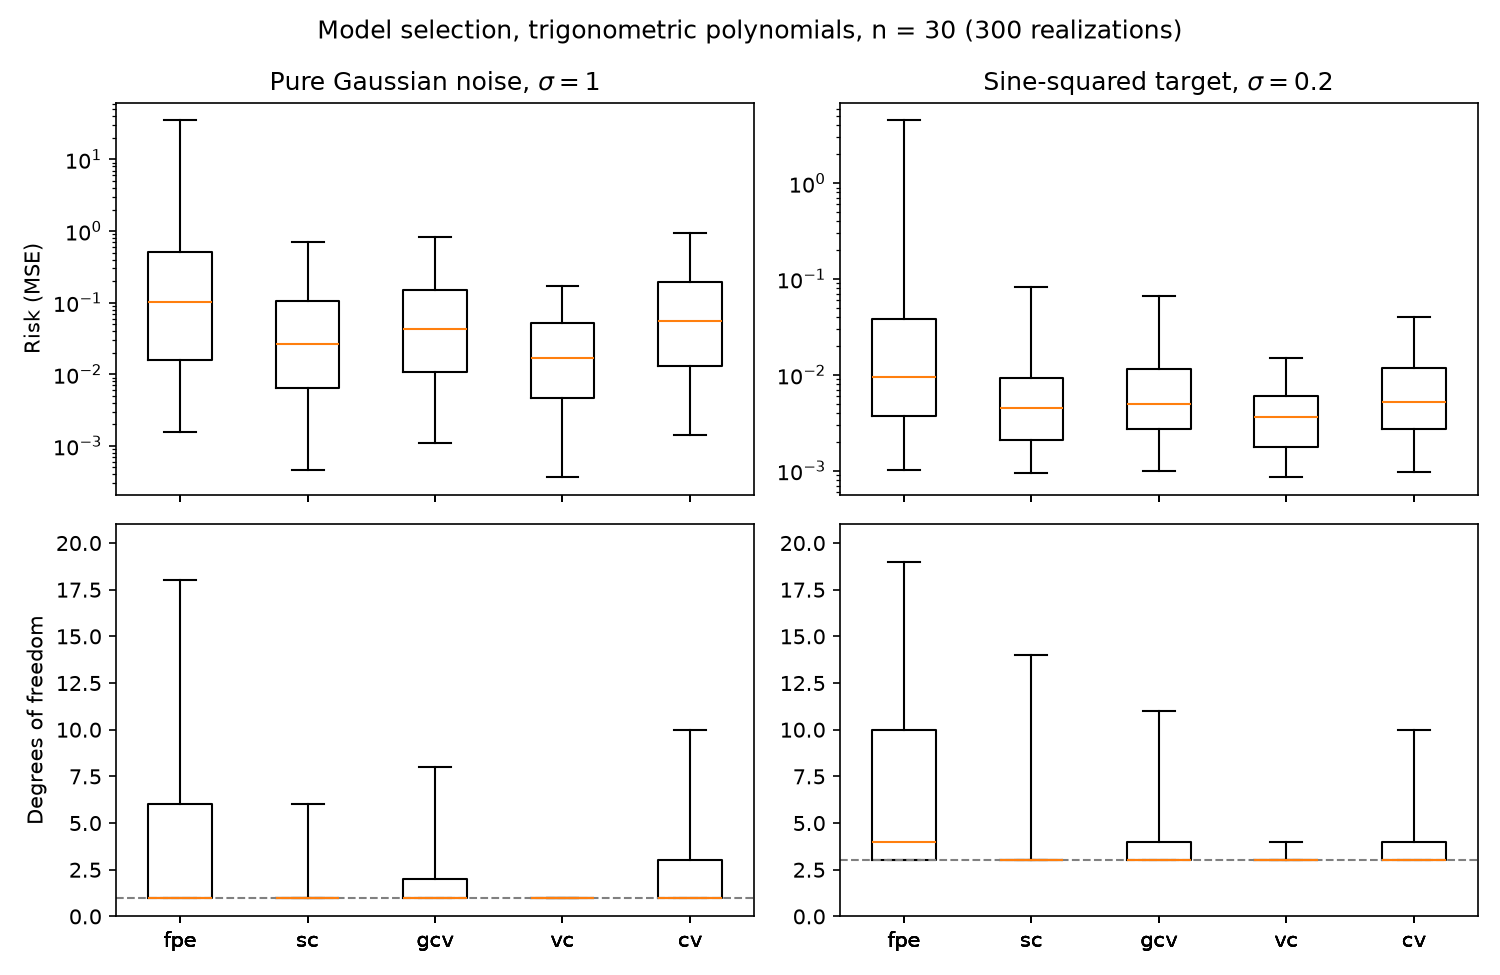
\includegraphics[width=0.92\linewidth]{p1_n30.png}
  \caption{Model selection results for $n = 30$ (300 realizations). Top: prediction risk (log scale);
           bottom: selected DoF. Left: pure noise; right: sine-squared.}
  \label{fig:p1n30}
\end{figure}

\begin{figure}[H]
  \centering
  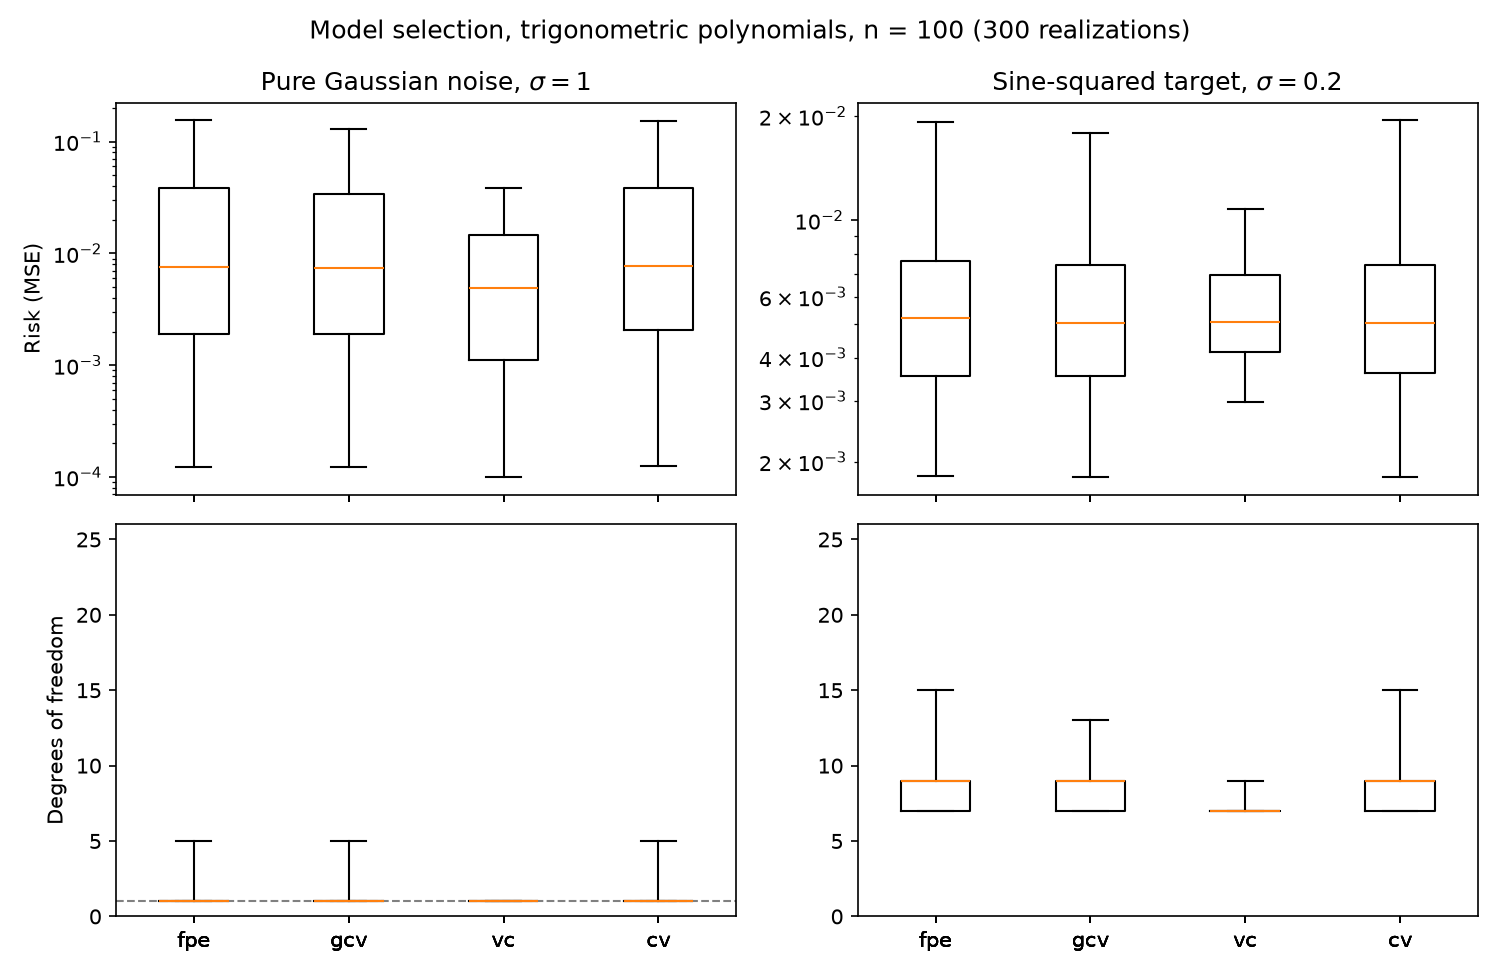
\includegraphics[width=0.92\linewidth]{p1_n100.png}
  \caption{Model selection results for $n = 100$ (300 realizations), same layout as Figure~\ref{fig:p1n30}.}
  \label{fig:p1n100}
\end{figure}

\begin{center}\small
\begin{tabular}{l rr rr rr rr}
\toprule
 & \multicolumn{4}{c}{$n = 30$} & \multicolumn{4}{c}{$n = 100$} \\
\cmidrule(lr){2-5}\cmidrule(lr){6-9}
 & \multicolumn{2}{c}{Pure noise} & \multicolumn{2}{c}{Sine-squared}
 & \multicolumn{2}{c}{Pure noise} & \multicolumn{2}{c}{Sine-squared} \\
Method & correct & risk p95 & correct & risk p95 & correct & risk p95 & correct & risk p95 \\
\midrule
fpe & 53.0\% & 35.7   & 46.3\% & 4.54   & 73.0\%  & 0.197  & 68.7\% & 0.0087 \\
sc  & 82.7\% & 0.708  & 76.0\% & 0.0821 & 95.3\%  & 0.0568 & 97.0\% & 0.0035 \\
gcv & 69.0\% & 0.831  & 67.7\% & 0.0672 & 74.0\%  & 0.134  & 73.0\% & 0.0063 \\
vc  & 97.7\% & 0.170  & 92.3\% & 0.0149 & 100.0\% & 0.0381 & 99.3\% & 0.0032 \\
cv  & 64.7\% & 0.945  & 64.7\% & 0.0402 & 74.7\%  & 0.132  & 74.3\% & 0.0060 \\
\bottomrule
\end{tabular}

\smallskip
\emph{correct}: share of the 300 realizations that selected the true DoF; \emph{risk p95}: 95th percentile of the prediction risk.
\end{center}

\paragraph{Small samples ($n = 30$).}
The share of correct selections follows the strength of the penalty: vc (97.7\% for pure noise, 92.3\% for
sine-squared) $>$ sc $>$ gcv $>$ cv $>$ fpe (53.0\%, 46.3\%). For sine-squared, fpe is the one method with a wrong
median DoF (4 instead of 3). Its light penalty lets a large drop in training error win: in one sine-squared sample,
fpe chose DoF $= 18$ while the other four methods chose DoF $= 3$. The tails of the risk distribution show the
largest gaps. For pure noise, the 95th-percentile risk of fpe (35.7) is about 200 times that of vc (0.17), while
their medians differ by a factor of six (0.103 vs.\ 0.017). In its worst 5\% of realizations, fpe picked models with
DoF 11--20, which swing far from zero between the training points; the worst vc selections had DoF 1 or 2.

\paragraph{Effect of sample size ($n = 100$).}
With $n = 100$, every method improves. vc selects the correct DoF in 100\% (pure noise) and 99.3\% (sine-squared) of
realizations, and sc in 95.3\% and 97.0\%. fpe, gcv, and cv level off at 70--75\%. For small $p$, these three
criteria charge about $2\sigma^2/n$ for each extra parameter, and a spurious term beats that charge with a probability
that does not shrink as $n$ grows. The sc charge, about $(\ln n)\,\sigma^2/n$, grows with $n$. The 95th-percentile
risk of fpe falls from 35.7 to 0.197 as its 95th-percentile DoF drops to 9 (pure noise) and 12 (sine-squared).

\subsection*{Conclusion}
Across both data sets and both sample sizes, the VC penalization chose the correct model most often and had the
lowest 95th-percentile risk. Its lead is widest at $n = 30$, where a wrong choice costs the most. The five methods
have similar median risks and separate in the worst 5\% of realizations, so a fair comparison needs the full risk
distribution.
.
% main.tex loads amsmath, graphicx, booktabs, float and sets
% \graphicspath{{../practice/}} (figures: p1_n30.png, p1_n100.png).
% All numbers come from HW2/practice/p1_mine.py (300 realizations, seed 0).
% ============================================================

\section*{Problem 1: Model selection for trigonometric polynomial regression}

\subsection*{Experimental setup}
I follow the procedure of Section~4.4 and compare analytic model selection criteria for univariate regression
with trigonometric polynomials
\[
  f_m(x) = w_0 + \sum_{k=1}^{m} w_k \cos(2\pi k x), \qquad \text{DoF} = m + 1,
\]
fitted by ordinary least squares. I draw inputs from $x \sim U[0,1]$ and use two data sets:
\begin{itemize}
  \item \textbf{Pure noise:} $y \sim N(0, 1)$. The true function is $f(x) = 0$, so the correct model is a constant (DoF $= 1$).
  \item \textbf{Sine-squared:} $y = \sin^2(2\pi x) + \varepsilon$, $\varepsilon \sim N(0, 0.2^2)$.
        Since $\sin^2(2\pi x) = \tfrac12 - \tfrac12\cos(4\pi x)$, the target belongs to the model with $m = 2$, and the correct DoF is 3.
\end{itemize}
I run 300 independent realizations for $n = 30$ (candidate DoF $1$--$20$) and $n = 100$ (candidate DoF $1$--$25$).
In each realization, every method selects a DoF. I refit the model with that DoF and measure its \emph{prediction
risk} as the mean squared error between the fitted model and the \emph{noise-free} target on 2000 independent test
points. No model can predict the noise, so this risk measures the distance between the selected model and the truth.

\subsection*{Model selection methods}
Training error falls as complexity grows, so it cannot guide model selection by itself. In one sine-squared sample
with $n = 30$, the training MSE fell from 0.107 at DoF $= 1$ to 0.0067 at DoF $= 20$, below the noise variance
$\sigma^2 = 0.04$. Each analytic method multiplies the training error $R_{\text{emp}}$ by a penalization factor
$r(p)$, where $p = \text{DoF}/n$, and selects the DoF that minimizes $r(p)\,R_{\text{emp}}$:
\begin{center}\small
\begin{tabular}{lll}
\toprule
Method & Penalization factor $r(p)$ & Reference \\
\midrule
Final prediction error (fpe) & $(1+p)/(1-p)$ & Eq.~(2.11) \\
Schwartz criterion (sc) & $1 + (\ln n)\, p/(1-p)$ & Eq.~(2.12) \\
Generalized cross-validation (gcv) & $(1-p)^{-2}$ & Eq.~(2.13) \\
VC bound (vc) & $\bigl(1 - \sqrt{p - p\ln p + \ln n/(2n)}\bigr)_+^{-1}$ & Eq.~(4.15) \\
\bottomrule
\end{tabular}
\end{center}
For vc, I set the factor to infinity when the term under the square root reaches 1, which excludes that model.
At $p = 0.1$ the four factors lie between 1.2 and 1.5. At $p = 0.5$ with $n = 30$ they spread out: fpe gives 3.0,
gcv 4.0, sc 4.4, and vc 20.2.

The fifth method, leave-one-out cross-validation (cv), estimates prediction risk from held-out data. I compute the
leave-one-out error from a single fit with the leverage formula $e_i/(1 - h_{ii})$, where $e_i$ is the ordinary
residual and $h_{ii}$ the $i$-th diagonal entry of the hat matrix. In my checks it matched the result of $n$
explicit refits to four decimal places.

\subsection*{Results}
Figures~\ref{fig:p1n30} and~\ref{fig:p1n100} present the results in the style of Figs.~4.10--4.11. Each box spans
the 25th to 75th percentiles with a line at the median, and the whiskers reach the 5th and 95th percentiles. The risk
panels use a logarithmic scale, and a dashed line in the DoF panels marks the correct DoF.

\begin{figure}[H]
  \centering
  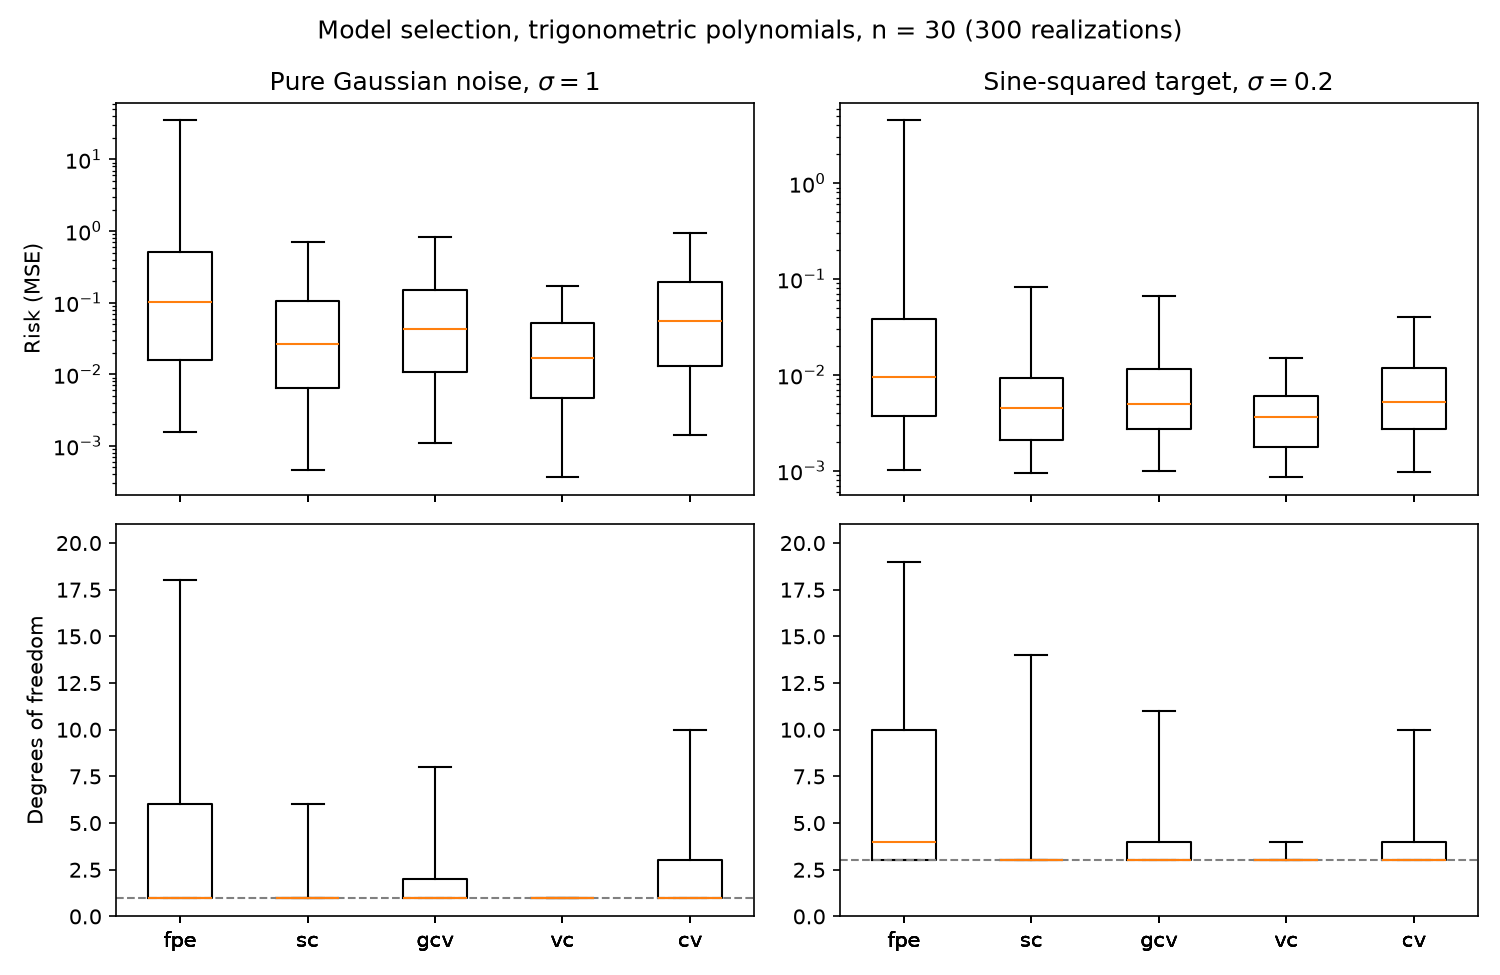
\includegraphics[width=0.92\linewidth]{p1_n30.png}
  \caption{Model selection results for $n = 30$ (300 realizations). Top: prediction risk (log scale);
           bottom: selected DoF. Left: pure noise; right: sine-squared.}
  \label{fig:p1n30}
\end{figure}

\begin{figure}[H]
  \centering
  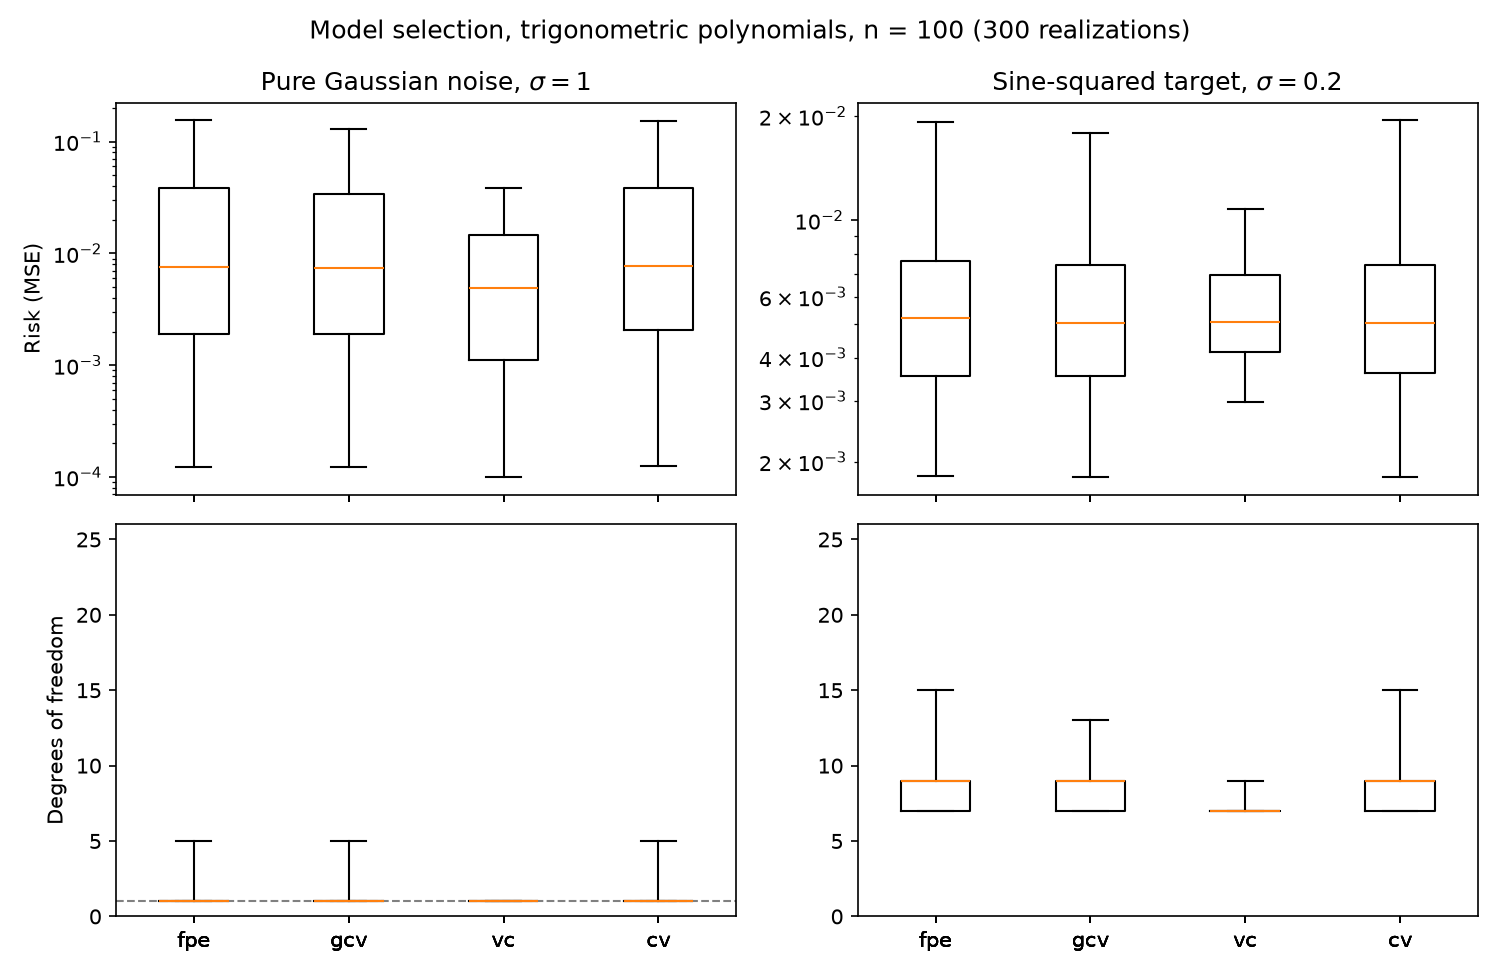
\includegraphics[width=0.92\linewidth]{p1_n100.png}
  \caption{Model selection results for $n = 100$ (300 realizations), same layout as Figure~\ref{fig:p1n30}.}
  \label{fig:p1n100}
\end{figure}

\begin{center}\small
\begin{tabular}{l rr rr rr rr}
\toprule
 & \multicolumn{4}{c}{$n = 30$} & \multicolumn{4}{c}{$n = 100$} \\
\cmidrule(lr){2-5}\cmidrule(lr){6-9}
 & \multicolumn{2}{c}{Pure noise} & \multicolumn{2}{c}{Sine-squared}
 & \multicolumn{2}{c}{Pure noise} & \multicolumn{2}{c}{Sine-squared} \\
Method & correct & risk p95 & correct & risk p95 & correct & risk p95 & correct & risk p95 \\
\midrule
fpe & 53.0\% & 35.7   & 46.3\% & 4.54   & 73.0\%  & 0.197  & 68.7\% & 0.0087 \\
sc  & 82.7\% & 0.708  & 76.0\% & 0.0821 & 95.3\%  & 0.0568 & 97.0\% & 0.0035 \\
gcv & 69.0\% & 0.831  & 67.7\% & 0.0672 & 74.0\%  & 0.134  & 73.0\% & 0.0063 \\
vc  & 97.7\% & 0.170  & 92.3\% & 0.0149 & 100.0\% & 0.0381 & 99.3\% & 0.0032 \\
cv  & 64.7\% & 0.945  & 64.7\% & 0.0402 & 74.7\%  & 0.132  & 74.3\% & 0.0060 \\
\bottomrule
\end{tabular}

\smallskip
\emph{correct}: share of the 300 realizations that selected the true DoF; \emph{risk p95}: 95th percentile of the prediction risk.
\end{center}

\paragraph{Small samples ($n = 30$).}
The share of correct selections follows the strength of the penalty: vc (97.7\% for pure noise, 92.3\% for
sine-squared) $>$ sc $>$ gcv $>$ cv $>$ fpe (53.0\%, 46.3\%). For sine-squared, fpe is the one method with a wrong
median DoF (4 instead of 3). Its light penalty lets a large drop in training error win: in one sine-squared sample,
fpe chose DoF $= 18$ while the other four methods chose DoF $= 3$. The tails of the risk distribution show the
largest gaps. For pure noise, the 95th-percentile risk of fpe (35.7) is about 200 times that of vc (0.17), while
their medians differ by a factor of six (0.103 vs.\ 0.017). In its worst 5\% of realizations, fpe picked models with
DoF 11--20, which swing far from zero between the training points; the worst vc selections had DoF 1 or 2.

\paragraph{Effect of sample size ($n = 100$).}
With $n = 100$, every method improves. vc selects the correct DoF in 100\% (pure noise) and 99.3\% (sine-squared) of
realizations, and sc in 95.3\% and 97.0\%. fpe, gcv, and cv level off at 70--75\%. For small $p$, these three
criteria charge about $2\sigma^2/n$ for each extra parameter, and a spurious term beats that charge with a probability
that does not shrink as $n$ grows. The sc charge, about $(\ln n)\,\sigma^2/n$, grows with $n$. The 95th-percentile
risk of fpe falls from 35.7 to 0.197 as its 95th-percentile DoF drops to 9 (pure noise) and 12 (sine-squared).

\subsection*{Conclusion}
Across both data sets and both sample sizes, the VC penalization chose the correct model most often and had the
lowest 95th-percentile risk. Its lead is widest at $n = 30$, where a wrong choice costs the most. The five methods
have similar median risks and separate in the worst 5\% of realizations, so a fair comparison needs the full risk
distribution.
.
% main.tex loads amsmath, graphicx, booktabs, float and sets
% \graphicspath{{../practice/}} (figures: p1_n30.png, p1_n100.png).
% All numbers come from HW2/practice/p1_mine.py (300 realizations, seed 0).
% ============================================================

\section*{Problem 1: Model selection for trigonometric polynomial regression}

\subsection*{Experimental setup}
I follow the procedure of Section~4.4 and compare analytic model selection criteria for univariate regression
with trigonometric polynomials
\[
  f_m(x) = w_0 + \sum_{k=1}^{m} w_k \cos(2\pi k x), \qquad \text{DoF} = m + 1,
\]
fitted by ordinary least squares. I draw inputs from $x \sim U[0,1]$ and use two data sets:
\begin{itemize}
  \item \textbf{Pure noise:} $y \sim N(0, 1)$. The true function is $f(x) = 0$, so the correct model is a constant (DoF $= 1$).
  \item \textbf{Sine-squared:} $y = \sin^2(2\pi x) + \varepsilon$, $\varepsilon \sim N(0, 0.2^2)$.
        Since $\sin^2(2\pi x) = \tfrac12 - \tfrac12\cos(4\pi x)$, the target belongs to the model with $m = 2$, and the correct DoF is 3.
\end{itemize}
I run 300 independent realizations for $n = 30$ (candidate DoF $1$--$20$) and $n = 100$ (candidate DoF $1$--$25$).
In each realization, every method selects a DoF. I refit the model with that DoF and measure its \emph{prediction
risk} as the mean squared error between the fitted model and the \emph{noise-free} target on 2000 independent test
points. No model can predict the noise, so this risk measures the distance between the selected model and the truth.

\subsection*{Model selection methods}
Training error falls as complexity grows, so it cannot guide model selection by itself. In one sine-squared sample
with $n = 30$, the training MSE fell from 0.107 at DoF $= 1$ to 0.0067 at DoF $= 20$, below the noise variance
$\sigma^2 = 0.04$. Each analytic method multiplies the training error $R_{\text{emp}}$ by a penalization factor
$r(p)$, where $p = \text{DoF}/n$, and selects the DoF that minimizes $r(p)\,R_{\text{emp}}$:
\begin{center}\small
\begin{tabular}{lll}
\toprule
Method & Penalization factor $r(p)$ & Reference \\
\midrule
Final prediction error (fpe) & $(1+p)/(1-p)$ & Eq.~(2.11) \\
Schwartz criterion (sc) & $1 + (\ln n)\, p/(1-p)$ & Eq.~(2.12) \\
Generalized cross-validation (gcv) & $(1-p)^{-2}$ & Eq.~(2.13) \\
VC bound (vc) & $\bigl(1 - \sqrt{p - p\ln p + \ln n/(2n)}\bigr)_+^{-1}$ & Eq.~(4.15) \\
\bottomrule
\end{tabular}
\end{center}
For vc, I set the factor to infinity when the term under the square root reaches 1, which excludes that model.
At $p = 0.1$ the four factors lie between 1.2 and 1.5. At $p = 0.5$ with $n = 30$ they spread out: fpe gives 3.0,
gcv 4.0, sc 4.4, and vc 20.2.

The fifth method, leave-one-out cross-validation (cv), estimates prediction risk from held-out data. I compute the
leave-one-out error from a single fit with the leverage formula $e_i/(1 - h_{ii})$, where $e_i$ is the ordinary
residual and $h_{ii}$ the $i$-th diagonal entry of the hat matrix. In my checks it matched the result of $n$
explicit refits to four decimal places.

\subsection*{Results}
Figures~\ref{fig:p1n30} and~\ref{fig:p1n100} present the results in the style of Figs.~4.10--4.11. Each box spans
the 25th to 75th percentiles with a line at the median, and the whiskers reach the 5th and 95th percentiles. The risk
panels use a logarithmic scale, and a dashed line in the DoF panels marks the correct DoF.

\begin{figure}[H]
  \centering
  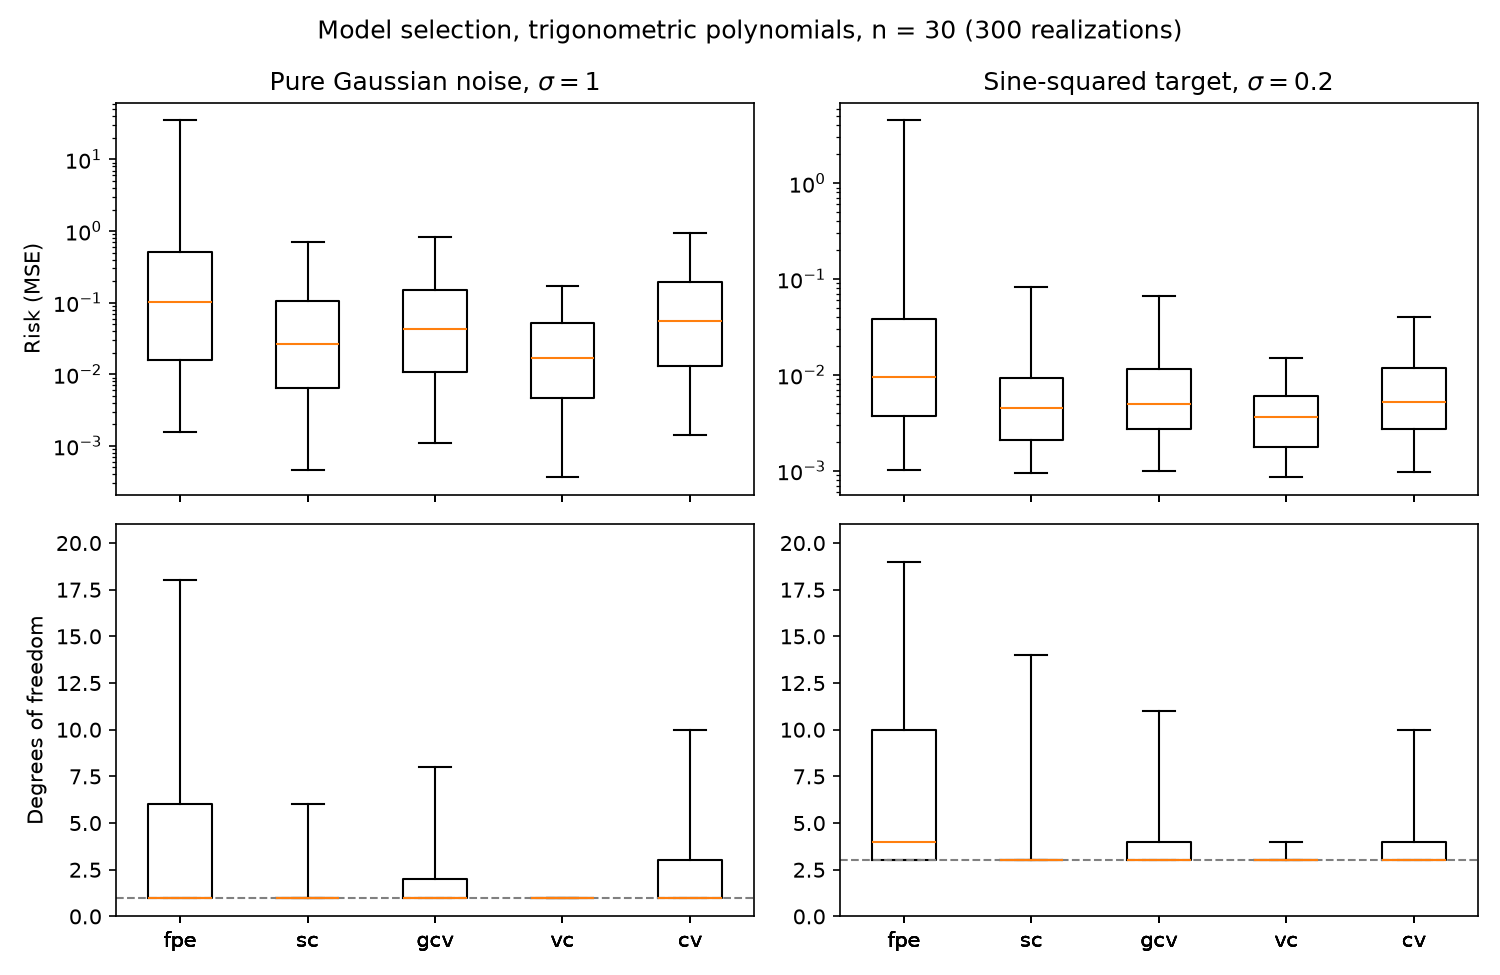
\includegraphics[width=0.92\linewidth]{p1_n30.png}
  \caption{Model selection results for $n = 30$ (300 realizations). Top: prediction risk (log scale);
           bottom: selected DoF. Left: pure noise; right: sine-squared.}
  \label{fig:p1n30}
\end{figure}

\begin{figure}[H]
  \centering
  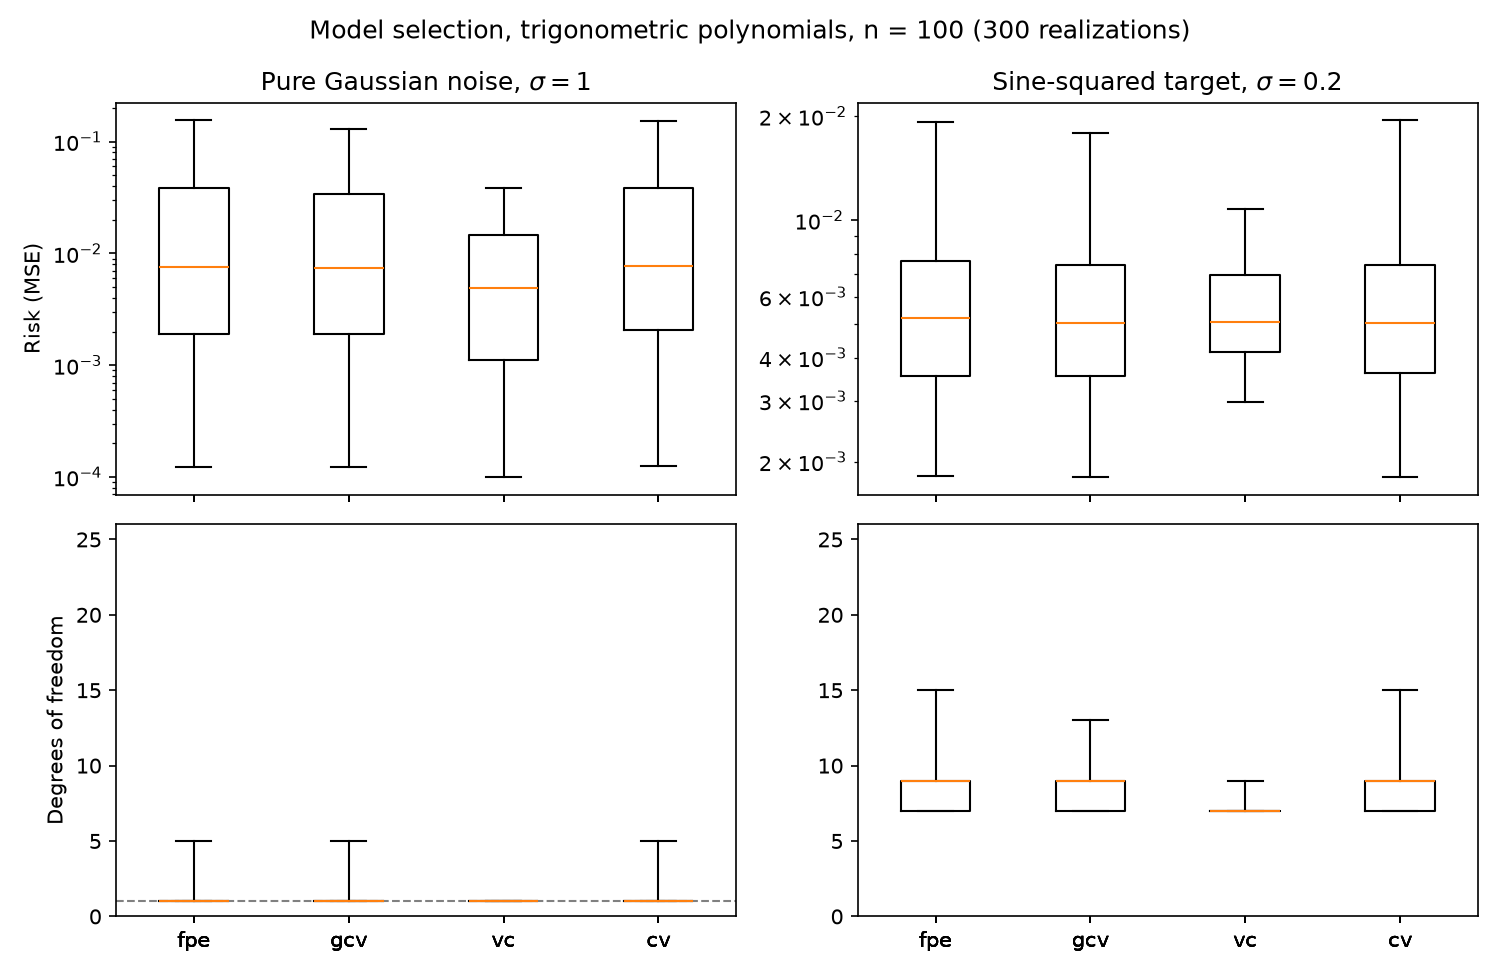
\includegraphics[width=0.92\linewidth]{p1_n100.png}
  \caption{Model selection results for $n = 100$ (300 realizations), same layout as Figure~\ref{fig:p1n30}.}
  \label{fig:p1n100}
\end{figure}

\begin{center}\small
\begin{tabular}{l rr rr rr rr}
\toprule
 & \multicolumn{4}{c}{$n = 30$} & \multicolumn{4}{c}{$n = 100$} \\
\cmidrule(lr){2-5}\cmidrule(lr){6-9}
 & \multicolumn{2}{c}{Pure noise} & \multicolumn{2}{c}{Sine-squared}
 & \multicolumn{2}{c}{Pure noise} & \multicolumn{2}{c}{Sine-squared} \\
Method & correct & risk p95 & correct & risk p95 & correct & risk p95 & correct & risk p95 \\
\midrule
fpe & 53.0\% & 35.7   & 46.3\% & 4.54   & 73.0\%  & 0.197  & 68.7\% & 0.0087 \\
sc  & 82.7\% & 0.708  & 76.0\% & 0.0821 & 95.3\%  & 0.0568 & 97.0\% & 0.0035 \\
gcv & 69.0\% & 0.831  & 67.7\% & 0.0672 & 74.0\%  & 0.134  & 73.0\% & 0.0063 \\
vc  & 97.7\% & 0.170  & 92.3\% & 0.0149 & 100.0\% & 0.0381 & 99.3\% & 0.0032 \\
cv  & 64.7\% & 0.945  & 64.7\% & 0.0402 & 74.7\%  & 0.132  & 74.3\% & 0.0060 \\
\bottomrule
\end{tabular}

\smallskip
\emph{correct}: share of the 300 realizations that selected the true DoF; \emph{risk p95}: 95th percentile of the prediction risk.
\end{center}

\paragraph{Small samples ($n = 30$).}
The share of correct selections follows the strength of the penalty: vc (97.7\% for pure noise, 92.3\% for
sine-squared) $>$ sc $>$ gcv $>$ cv $>$ fpe (53.0\%, 46.3\%). For sine-squared, fpe is the one method with a wrong
median DoF (4 instead of 3). Its light penalty lets a large drop in training error win: in one sine-squared sample,
fpe chose DoF $= 18$ while the other four methods chose DoF $= 3$. The tails of the risk distribution show the
largest gaps. For pure noise, the 95th-percentile risk of fpe (35.7) is about 200 times that of vc (0.17), while
their medians differ by a factor of six (0.103 vs.\ 0.017). In its worst 5\% of realizations, fpe picked models with
DoF 11--20, which swing far from zero between the training points; the worst vc selections had DoF 1 or 2.

\paragraph{Effect of sample size ($n = 100$).}
With $n = 100$, every method improves. vc selects the correct DoF in 100\% (pure noise) and 99.3\% (sine-squared) of
realizations, and sc in 95.3\% and 97.0\%. fpe, gcv, and cv level off at 70--75\%. For small $p$, these three
criteria charge about $2\sigma^2/n$ for each extra parameter, and a spurious term beats that charge with a probability
that does not shrink as $n$ grows. The sc charge, about $(\ln n)\,\sigma^2/n$, grows with $n$. The 95th-percentile
risk of fpe falls from 35.7 to 0.197 as its 95th-percentile DoF drops to 9 (pure noise) and 12 (sine-squared).

\subsection*{Conclusion}
Across both data sets and both sample sizes, the VC penalization chose the correct model most often and had the
lowest 95th-percentile risk. Its lead is widest at $n = 30$, where a wrong choice costs the most. The five methods
have similar median risks and separate in the worst 5\% of realizations, so a fair comparison needs the full risk
distribution.


% ============================================================
% Problem 2 section of the combined HW2 report (Problems 1 + 2).
% This is a fragment, included from HW2/report/main.tex via % ============================================================
% Problem 2 section of the combined HW2 report (Problems 1 + 2).
% This is a fragment, included from HW2/report/main.tex via % ============================================================
% Problem 2 section of the combined HW2 report (Problems 1 + 2).
% This is a fragment, included from HW2/report/main.tex via \input{problem2}.
% Figure: p2_boundaries.png (found through \graphicspath{{../practice/}}).
% All numbers come from HW2/practice/p2_mine.py; the 2003-12-31 prices are in
% HW2/data/extra_2003-12-31.csv.
% ============================================================

\section*{Problem 2: Trading international mutual funds}

\subsection*{Data and encoding}
I use daily closing prices of the S\&P 500 (\texttt{\^{}GSPC}) and the Fidelity International Discovery fund
(FIGRX) from Yahoo Finance, and the euro exchange rate (euros per US dollar) from the UBC Pacific Exchange Rate
Service. Following the course preprocessing note, I keep the dates present in all three series: 243 trading days in
2004 and 245 in 2005. Alignment removes nine 2004 days on which the UBC file has no quote, most of them Canadian
holidays, and seven US market holidays on which it does.

The inputs are today's percentage changes, $x_1$ for the S\&P 500 and $x_2$ for the exchange rate, each measured
against the previous aligned day. The output $y$ is tomorrow's percentage change of FIGRX. I join the price series
across years to compute the changes at the year boundaries. The output for December 31, 2004 uses the first aligned
day of 2005 (January 4). The input for January 6, 2004, the first aligned day of that year, needs the close of
December 31, 2003, which the provided files do not contain; I retrieved the three values from the same sources
(S\&P 500 1111.92, FIGRX 23.92, 0.79386 euros per dollar). I obtain 243 training samples (January 6 to
December 31, 2004) and 244 test samples (January 4 to December 29, 2005). The last day of 2005 has no next-day
output.

FIGRX closed unchanged on seven 2004 days. I drop those days when I fit the quadratic classifier and when I
compute accuracy. The trading simulation keeps them: a zero change produces zero gain under either position.

\subsection*{Classifiers}
\paragraph{(a) Linear classifier.}
I fit $t(\mathbf{x}) = w_0 + w_1 x_1 + w_2 x_2$ to the real-valued outputs by least squares and predict UP when
$t(\mathbf{x}) > 0$. The 2004 data give
\[
  t(\mathbf{x}) = 0.0469 + 0.0844\,x_1 - 0.0073\,x_2 .
\]
The positive S\&P 500 coefficient fits the view that foreign markets follow the US market with a one-day lag. The
exchange-rate coefficient is close to zero. With a positive intercept, the rule predicts DOWN after the S\&P 500
falls by more than about 0.56\%, and it predicts UP on 79\% of training days.

\paragraph{(b) Quadratic classifier.}
I convert the outputs to class labels $y = \operatorname{sign}(y)$ and fit
\[
  g(\mathbf{x}, \mathbf{w}) = w_1 x_1 + w_2 x_2 + w_3 x_1^2 + w_4 x_2^2 + w_5 x_1 x_2 + w_0
\]
to the $\pm 1$ labels by least squares, then predict UP when $g > 0$. The assignment leaves the estimation method
open; least squares keeps the two approaches comparable. The fitted coefficients are $w_0 = 0.1594$,
$w_1 = 0.0787$, $w_2 = 0.1112$, $w_3 = -0.0606$, $w_4 = -0.1470$, and $w_5 = 0.1361$. The quadratic part is
negative definite ($w_3 < 0$ and $w_3 w_4 - w_5^2/4 = 0.0043 > 0$) and the intercept is positive, so the boundary is
an ellipse with the UP region inside. The model predicts UP on calm days and DOWN after large moves in either input.

\begin{center}\small
\begin{tabular}{lcc}
\toprule
Classifier & Training accuracy (2004) & Test accuracy (2005) \\
\midrule
Linear & 51.7\% & 57.1\% \\
Quadratic & 57.2\% & 55.8\% \\
Always UP & 52.5\% & 55.0\% \\
\bottomrule
\end{tabular}
\end{center}

The quadratic model gains 5.5 points of training accuracy over the linear one and loses 1.3 points on the test year,
a pattern consistent with overfitting. The two models also differ in their fitting target (real-valued changes versus
$\pm 1$ labels), so this comparison mixes complexity with the choice of target. With about 240 days per year, one day
moves accuracy by 0.4 points, and the standard error of an accuracy estimate is close to 3 points. Neither classifier beats the always-UP rule by more
than that margin.

\subsection*{Decision boundaries}
Figure~\ref{fig:p2boundaries} plots both boundaries over the training and test data in the required
$(-2\%, +2\%)$ range. The linear boundary runs close to vertical at $x_1 \approx -0.56\%$, because the exchange rate
carries almost no weight. The quadratic ellipse tilts toward the upper right and extends past the plotted range. Its
lower edge near $x_2 = -0.7\%$ wraps around a group of 2004 DOWN days that has no counterpart in 2005. In all four
panels the UP and DOWN days overlap, and no boundary of either shape separates them.

\begin{figure}[htbp]
  \centering
  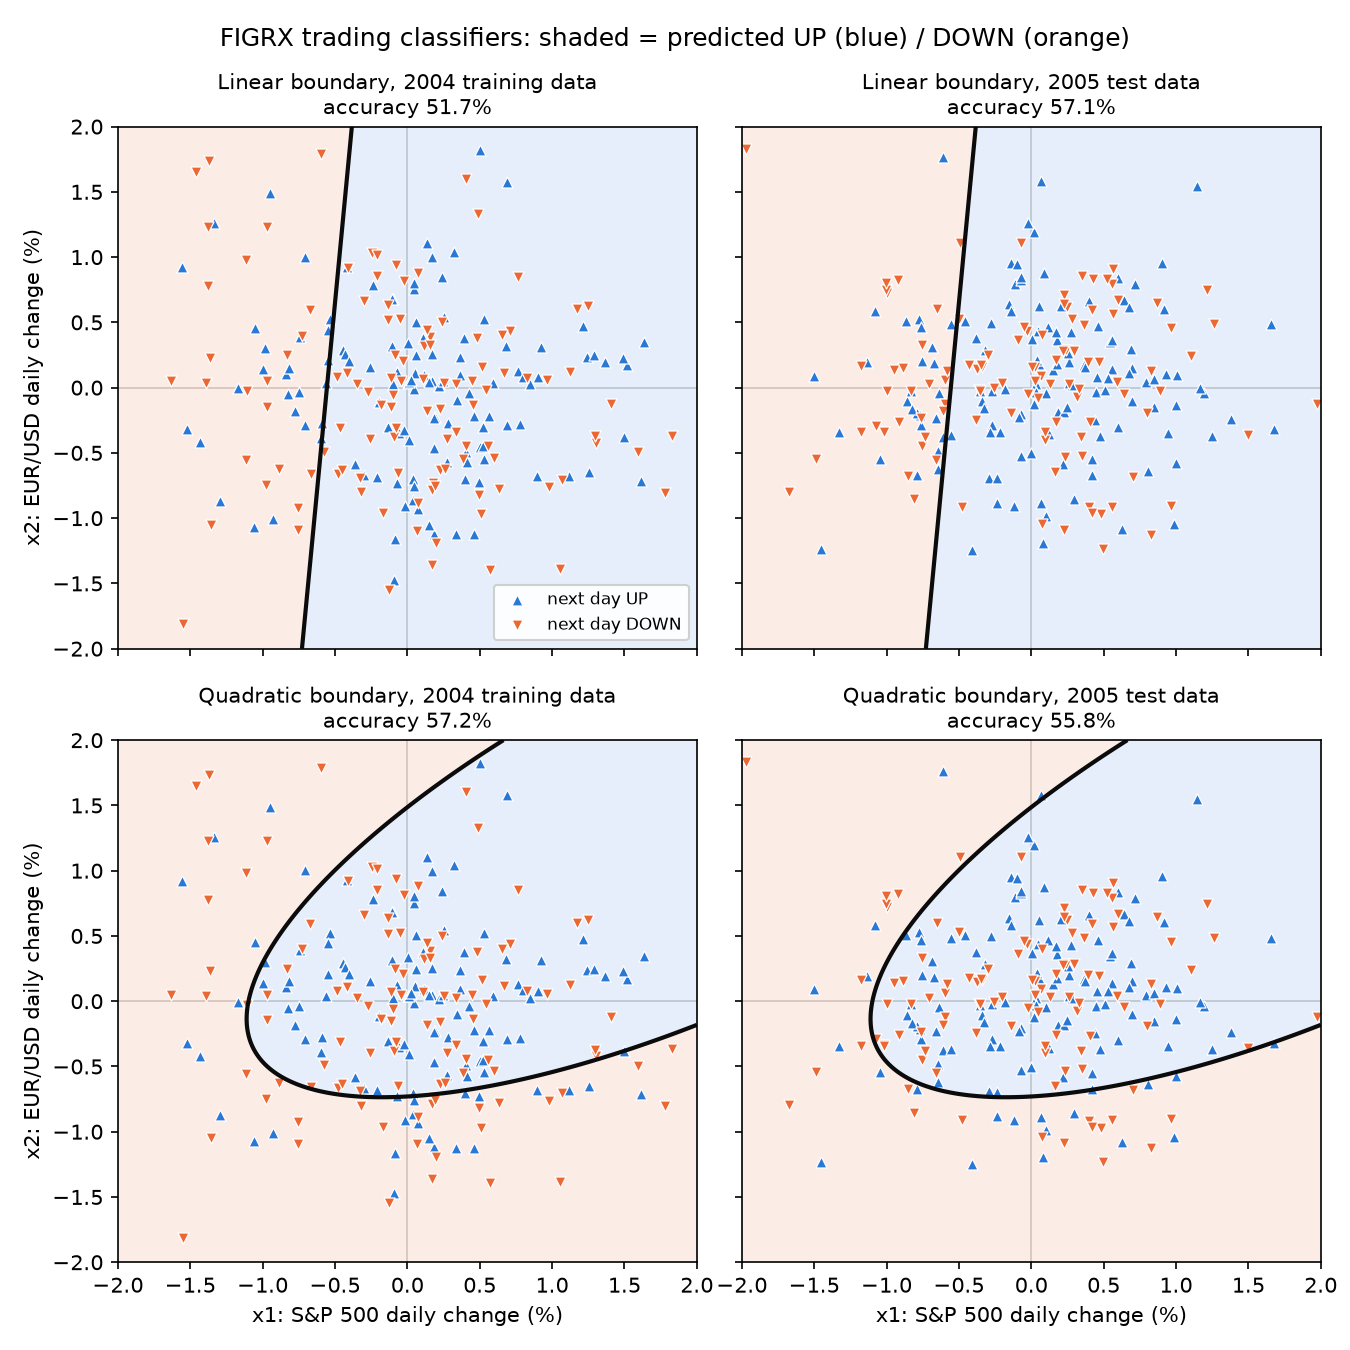
\includegraphics[width=0.8\linewidth]{p2_boundaries.png}
  \caption{Decision boundaries of the linear (top) and quadratic (bottom) classifiers over the 2004 training data
           (left) and the 2005 test data (right). Shading shows the predicted class; markers show the actual
           next-day FIGRX change.}
  \label{fig:p2boundaries}
\end{figure}

On 2005 days inside the ellipse, FIGRX rose the next day 56.6\% of the time, against 47.7\% outside. The outside
group holds 44 days, so its standard error is about 7.5 points, and the gap falls within sampling error. On the 2004
data used to fit the ellipse, the same comparison gave 56.7\% and 41.5\%.

\Needspace{14\baselineskip}
\subsection*{Trading results}
Each strategy holds FIGRX on days its classifier predicts UP and cash otherwise. Starting from \$1 million, I
compound the daily returns over the 2005 test period. GAIN is the cumulative return at the end of the year, and
EXPOSURE is the share of days invested in FIGRX.

\begin{center}\small
\begin{tabular}{lcc}
\toprule
Strategy & GAIN & EXPOSURE \\
\midrule
Linear & 21.81\% & 76.6\% \\
Quadratic & 15.19\% & 82.0\% \\
Buy-and-Hold & 14.92\% & 100.0\% \\
\bottomrule
\end{tabular}
\end{center}

Buy-and-Hold earns 14.92\%, from the January 4 close (27.55) to the December 30 close (31.66). The linear strategy
earns 6.9 points more while staying in cash on 57 days. On those days FIGRX moved $-0.10\%$ on average, against
$+0.11\%$ on the days the strategy held the fund. The gain depends on the size of each day's move, so a rule with a
small accuracy edge can earn more by skipping days with large declines. To judge luck, I drew 10{,}000 random strategies invested on the same 76.6\% of days. Their
median gain is 11.2\%, and 3.1\% of them reach 21.81\% or more.

\subsection*{Discussion}
\paragraph{(a) Can this strategy be used in practice?}
I would not trade my own money with it. The 2005 result rests on one test year, and I picked the better of two
models after seeing both. Neither classifier beats the always-UP rule in accuracy by more than the sampling error,
and the UP and DOWN days overlap across the input plane. A possible source of the linear rule's profit is the stale
pricing of international funds, whose prices use foreign closes that have not yet reacted to the US market; my
experiment does not test this mechanism. After the 2003 mutual-fund scandal, fund companies adopted fair-value
pricing, and many restrict short-term trading or charge redemption fees, which would close such a gap. The assignment
also assumes zero transaction costs. The linear strategy switches position 89 times in 2005. If each switch costs
0.1\% of the account, its gain falls from 21.81\% to 11.43\%, below the 14.92\% of Buy-and-Hold.

\paragraph{(b) VC-theoretical explanation.}
Problem 2 is a classification task with 0/1 loss, so the relevant result is the VC bound for classification. It
adds a confidence term $\Phi$ to the training error rate,
\[
  R(\omega) \le R_{\text{emp}}(\omega) + \Phi, \qquad
  \Phi = \sqrt{\frac{h\bigl(\ln(2n/h) + 1\bigr) - \ln(\eta/4)}{n}},
\]
and holds with probability at least $1 - \eta$. I set $\eta = \min(4/\sqrt{n}, 1)$, the textbook's practical rule,
which raises the confidence level as the sample grows. The multiplicative VC penalization factor used in Problem 1
belongs to regression. Each classifier is linear in its parameters, so its VC-dimension equals the parameter count:
$h = 3$ for the linear rule and $h = 6$ for the quadratic rule. A VC bound holds for every function in the model
set, so it also covers my least-squares classifiers, which do not minimize the 0/1 training error.

\begin{center}\small
\begin{tabular}{lcccccc}
\toprule
Classifier & $h$ & $n$ & $n/h$ & $R_{\text{emp}}$ & $\Phi$ & Upper bound on $R$ \\
\midrule
Linear & 3 & 236 & 78.7 & 0.483 & 0.298 & 0.781 \\
Quadratic & 6 & 236 & 39.3 & 0.428 & 0.385 & 0.813 \\
\bottomrule
\end{tabular}
\end{center}

The 0/1 training error uses the 236 days with a nonzero FIGRX change. With $n = 236$, the rule gives
$\eta = 4/\sqrt{236} \approx 0.26$, so the bounds hold with probability at least $1 - \eta \approx 74\%$, below the
95\% level common in statistics.

The textbook calls a sample small when $n/h$ is below about 15; in that regime $\Phi$ stays large, and model
selection has to match the complexity to the data. The
assignment fixes two low-capacity model sets in advance and fits each once, without searching over model sizes. Both
classifiers lie well above the small-sample threshold ($n/h$ of 78.7 and 39.3), which gives intuitive support for this
choice: further complexity control has less to gain here than in the small samples of Problem 1. This argument is a
heuristic, and a large $n/h$ leaves room for some benefit from complexity control.

Despite the large $n/h$, both upper bounds (0.781 and 0.813) exceed the 0.5 error of random guessing, so the theory
certifies no useful classifier from these 236 days. The training error rates sit near 0.5 before adding $\Phi$, and $\Phi$ needs a
large $n$ to become small, since its numerator also grows with $\ln n$. With $h = 3$ and the same rule for $\eta$,
$\Phi$ falls to about 0.06 only near $n = 10{,}000$ trading days.

The bound also assumes independent samples from one fixed distribution. Daily returns can depend on earlier days,
and the 2004 and 2005 markets need not share a distribution, so the bound gives a rough guide to the 2005 test error
at best. My results show that these two classifiers, with these two inputs, did not deliver a robust predictive
advantage in 2005; other models and other inputs remain untested.
.
% Figure: p2_boundaries.png (found through \graphicspath{{../practice/}}).
% All numbers come from HW2/practice/p2_mine.py; the 2003-12-31 prices are in
% HW2/data/extra_2003-12-31.csv.
% ============================================================

\section*{Problem 2: Trading international mutual funds}

\subsection*{Data and encoding}
I use daily closing prices of the S\&P 500 (\texttt{\^{}GSPC}) and the Fidelity International Discovery fund
(FIGRX) from Yahoo Finance, and the euro exchange rate (euros per US dollar) from the UBC Pacific Exchange Rate
Service. Following the course preprocessing note, I keep the dates present in all three series: 243 trading days in
2004 and 245 in 2005. Alignment removes nine 2004 days on which the UBC file has no quote, most of them Canadian
holidays, and seven US market holidays on which it does.

The inputs are today's percentage changes, $x_1$ for the S\&P 500 and $x_2$ for the exchange rate, each measured
against the previous aligned day. The output $y$ is tomorrow's percentage change of FIGRX. I join the price series
across years to compute the changes at the year boundaries. The output for December 31, 2004 uses the first aligned
day of 2005 (January 4). The input for January 6, 2004, the first aligned day of that year, needs the close of
December 31, 2003, which the provided files do not contain; I retrieved the three values from the same sources
(S\&P 500 1111.92, FIGRX 23.92, 0.79386 euros per dollar). I obtain 243 training samples (January 6 to
December 31, 2004) and 244 test samples (January 4 to December 29, 2005). The last day of 2005 has no next-day
output.

FIGRX closed unchanged on seven 2004 days. I drop those days when I fit the quadratic classifier and when I
compute accuracy. The trading simulation keeps them: a zero change produces zero gain under either position.

\subsection*{Classifiers}
\paragraph{(a) Linear classifier.}
I fit $t(\mathbf{x}) = w_0 + w_1 x_1 + w_2 x_2$ to the real-valued outputs by least squares and predict UP when
$t(\mathbf{x}) > 0$. The 2004 data give
\[
  t(\mathbf{x}) = 0.0469 + 0.0844\,x_1 - 0.0073\,x_2 .
\]
The positive S\&P 500 coefficient fits the view that foreign markets follow the US market with a one-day lag. The
exchange-rate coefficient is close to zero. With a positive intercept, the rule predicts DOWN after the S\&P 500
falls by more than about 0.56\%, and it predicts UP on 79\% of training days.

\paragraph{(b) Quadratic classifier.}
I convert the outputs to class labels $y = \operatorname{sign}(y)$ and fit
\[
  g(\mathbf{x}, \mathbf{w}) = w_1 x_1 + w_2 x_2 + w_3 x_1^2 + w_4 x_2^2 + w_5 x_1 x_2 + w_0
\]
to the $\pm 1$ labels by least squares, then predict UP when $g > 0$. The assignment leaves the estimation method
open; least squares keeps the two approaches comparable. The fitted coefficients are $w_0 = 0.1594$,
$w_1 = 0.0787$, $w_2 = 0.1112$, $w_3 = -0.0606$, $w_4 = -0.1470$, and $w_5 = 0.1361$. The quadratic part is
negative definite ($w_3 < 0$ and $w_3 w_4 - w_5^2/4 = 0.0043 > 0$) and the intercept is positive, so the boundary is
an ellipse with the UP region inside. The model predicts UP on calm days and DOWN after large moves in either input.

\begin{center}\small
\begin{tabular}{lcc}
\toprule
Classifier & Training accuracy (2004) & Test accuracy (2005) \\
\midrule
Linear & 51.7\% & 57.1\% \\
Quadratic & 57.2\% & 55.8\% \\
Always UP & 52.5\% & 55.0\% \\
\bottomrule
\end{tabular}
\end{center}

The quadratic model gains 5.5 points of training accuracy over the linear one and loses 1.3 points on the test year,
a pattern consistent with overfitting. The two models also differ in their fitting target (real-valued changes versus
$\pm 1$ labels), so this comparison mixes complexity with the choice of target. With about 240 days per year, one day
moves accuracy by 0.4 points, and the standard error of an accuracy estimate is close to 3 points. Neither classifier beats the always-UP rule by more
than that margin.

\subsection*{Decision boundaries}
Figure~\ref{fig:p2boundaries} plots both boundaries over the training and test data in the required
$(-2\%, +2\%)$ range. The linear boundary runs close to vertical at $x_1 \approx -0.56\%$, because the exchange rate
carries almost no weight. The quadratic ellipse tilts toward the upper right and extends past the plotted range. Its
lower edge near $x_2 = -0.7\%$ wraps around a group of 2004 DOWN days that has no counterpart in 2005. In all four
panels the UP and DOWN days overlap, and no boundary of either shape separates them.

\begin{figure}[htbp]
  \centering
  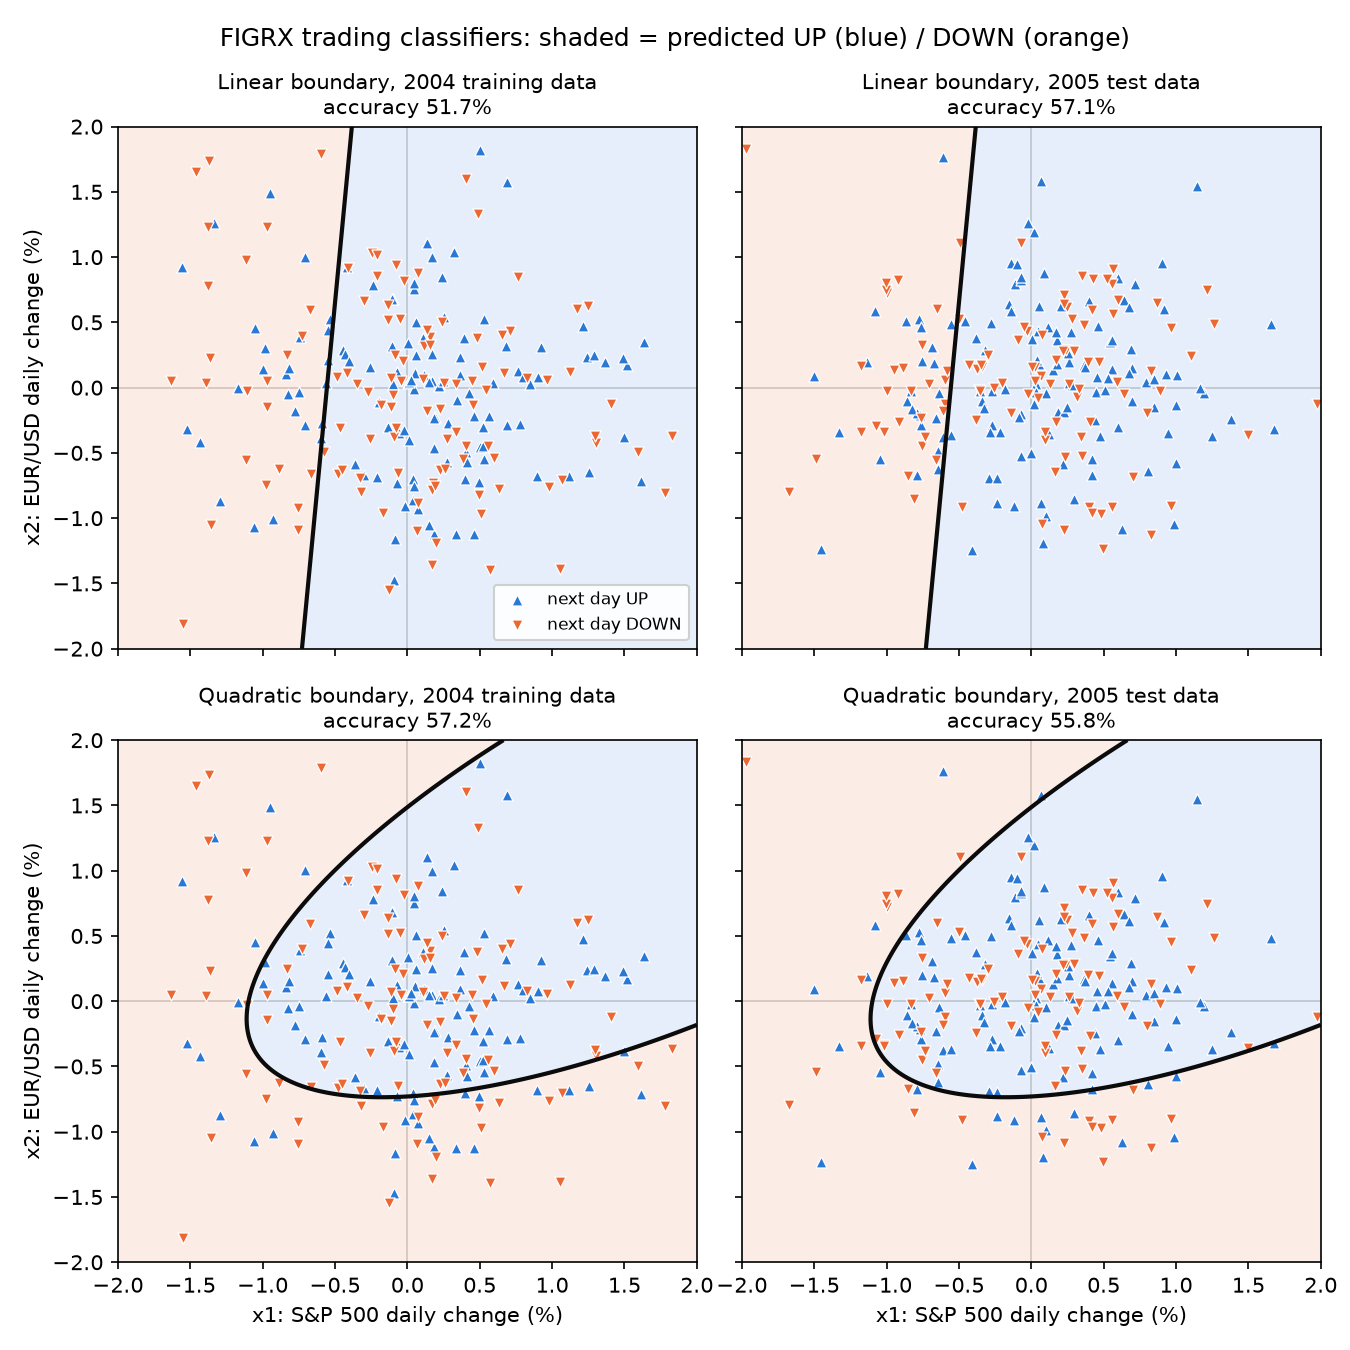
\includegraphics[width=0.8\linewidth]{p2_boundaries.png}
  \caption{Decision boundaries of the linear (top) and quadratic (bottom) classifiers over the 2004 training data
           (left) and the 2005 test data (right). Shading shows the predicted class; markers show the actual
           next-day FIGRX change.}
  \label{fig:p2boundaries}
\end{figure}

On 2005 days inside the ellipse, FIGRX rose the next day 56.6\% of the time, against 47.7\% outside. The outside
group holds 44 days, so its standard error is about 7.5 points, and the gap falls within sampling error. On the 2004
data used to fit the ellipse, the same comparison gave 56.7\% and 41.5\%.

\Needspace{14\baselineskip}
\subsection*{Trading results}
Each strategy holds FIGRX on days its classifier predicts UP and cash otherwise. Starting from \$1 million, I
compound the daily returns over the 2005 test period. GAIN is the cumulative return at the end of the year, and
EXPOSURE is the share of days invested in FIGRX.

\begin{center}\small
\begin{tabular}{lcc}
\toprule
Strategy & GAIN & EXPOSURE \\
\midrule
Linear & 21.81\% & 76.6\% \\
Quadratic & 15.19\% & 82.0\% \\
Buy-and-Hold & 14.92\% & 100.0\% \\
\bottomrule
\end{tabular}
\end{center}

Buy-and-Hold earns 14.92\%, from the January 4 close (27.55) to the December 30 close (31.66). The linear strategy
earns 6.9 points more while staying in cash on 57 days. On those days FIGRX moved $-0.10\%$ on average, against
$+0.11\%$ on the days the strategy held the fund. The gain depends on the size of each day's move, so a rule with a
small accuracy edge can earn more by skipping days with large declines. To judge luck, I drew 10{,}000 random strategies invested on the same 76.6\% of days. Their
median gain is 11.2\%, and 3.1\% of them reach 21.81\% or more.

\subsection*{Discussion}
\paragraph{(a) Can this strategy be used in practice?}
I would not trade my own money with it. The 2005 result rests on one test year, and I picked the better of two
models after seeing both. Neither classifier beats the always-UP rule in accuracy by more than the sampling error,
and the UP and DOWN days overlap across the input plane. A possible source of the linear rule's profit is the stale
pricing of international funds, whose prices use foreign closes that have not yet reacted to the US market; my
experiment does not test this mechanism. After the 2003 mutual-fund scandal, fund companies adopted fair-value
pricing, and many restrict short-term trading or charge redemption fees, which would close such a gap. The assignment
also assumes zero transaction costs. The linear strategy switches position 89 times in 2005. If each switch costs
0.1\% of the account, its gain falls from 21.81\% to 11.43\%, below the 14.92\% of Buy-and-Hold.

\paragraph{(b) VC-theoretical explanation.}
Problem 2 is a classification task with 0/1 loss, so the relevant result is the VC bound for classification. It
adds a confidence term $\Phi$ to the training error rate,
\[
  R(\omega) \le R_{\text{emp}}(\omega) + \Phi, \qquad
  \Phi = \sqrt{\frac{h\bigl(\ln(2n/h) + 1\bigr) - \ln(\eta/4)}{n}},
\]
and holds with probability at least $1 - \eta$. I set $\eta = \min(4/\sqrt{n}, 1)$, the textbook's practical rule,
which raises the confidence level as the sample grows. The multiplicative VC penalization factor used in Problem 1
belongs to regression. Each classifier is linear in its parameters, so its VC-dimension equals the parameter count:
$h = 3$ for the linear rule and $h = 6$ for the quadratic rule. A VC bound holds for every function in the model
set, so it also covers my least-squares classifiers, which do not minimize the 0/1 training error.

\begin{center}\small
\begin{tabular}{lcccccc}
\toprule
Classifier & $h$ & $n$ & $n/h$ & $R_{\text{emp}}$ & $\Phi$ & Upper bound on $R$ \\
\midrule
Linear & 3 & 236 & 78.7 & 0.483 & 0.298 & 0.781 \\
Quadratic & 6 & 236 & 39.3 & 0.428 & 0.385 & 0.813 \\
\bottomrule
\end{tabular}
\end{center}

The 0/1 training error uses the 236 days with a nonzero FIGRX change. With $n = 236$, the rule gives
$\eta = 4/\sqrt{236} \approx 0.26$, so the bounds hold with probability at least $1 - \eta \approx 74\%$, below the
95\% level common in statistics.

The textbook calls a sample small when $n/h$ is below about 15; in that regime $\Phi$ stays large, and model
selection has to match the complexity to the data. The
assignment fixes two low-capacity model sets in advance and fits each once, without searching over model sizes. Both
classifiers lie well above the small-sample threshold ($n/h$ of 78.7 and 39.3), which gives intuitive support for this
choice: further complexity control has less to gain here than in the small samples of Problem 1. This argument is a
heuristic, and a large $n/h$ leaves room for some benefit from complexity control.

Despite the large $n/h$, both upper bounds (0.781 and 0.813) exceed the 0.5 error of random guessing, so the theory
certifies no useful classifier from these 236 days. The training error rates sit near 0.5 before adding $\Phi$, and $\Phi$ needs a
large $n$ to become small, since its numerator also grows with $\ln n$. With $h = 3$ and the same rule for $\eta$,
$\Phi$ falls to about 0.06 only near $n = 10{,}000$ trading days.

The bound also assumes independent samples from one fixed distribution. Daily returns can depend on earlier days,
and the 2004 and 2005 markets need not share a distribution, so the bound gives a rough guide to the 2005 test error
at best. My results show that these two classifiers, with these two inputs, did not deliver a robust predictive
advantage in 2005; other models and other inputs remain untested.
.
% Figure: p2_boundaries.png (found through \graphicspath{{../practice/}}).
% All numbers come from HW2/practice/p2_mine.py; the 2003-12-31 prices are in
% HW2/data/extra_2003-12-31.csv.
% ============================================================

\section*{Problem 2: Trading international mutual funds}

\subsection*{Data and encoding}
I use daily closing prices of the S\&P 500 (\texttt{\^{}GSPC}) and the Fidelity International Discovery fund
(FIGRX) from Yahoo Finance, and the euro exchange rate (euros per US dollar) from the UBC Pacific Exchange Rate
Service. Following the course preprocessing note, I keep the dates present in all three series: 243 trading days in
2004 and 245 in 2005. Alignment removes nine 2004 days on which the UBC file has no quote, most of them Canadian
holidays, and seven US market holidays on which it does.

The inputs are today's percentage changes, $x_1$ for the S\&P 500 and $x_2$ for the exchange rate, each measured
against the previous aligned day. The output $y$ is tomorrow's percentage change of FIGRX. I join the price series
across years to compute the changes at the year boundaries. The output for December 31, 2004 uses the first aligned
day of 2005 (January 4). The input for January 6, 2004, the first aligned day of that year, needs the close of
December 31, 2003, which the provided files do not contain; I retrieved the three values from the same sources
(S\&P 500 1111.92, FIGRX 23.92, 0.79386 euros per dollar). I obtain 243 training samples (January 6 to
December 31, 2004) and 244 test samples (January 4 to December 29, 2005). The last day of 2005 has no next-day
output.

FIGRX closed unchanged on seven 2004 days. I drop those days when I fit the quadratic classifier and when I
compute accuracy. The trading simulation keeps them: a zero change produces zero gain under either position.

\subsection*{Classifiers}
\paragraph{(a) Linear classifier.}
I fit $t(\mathbf{x}) = w_0 + w_1 x_1 + w_2 x_2$ to the real-valued outputs by least squares and predict UP when
$t(\mathbf{x}) > 0$. The 2004 data give
\[
  t(\mathbf{x}) = 0.0469 + 0.0844\,x_1 - 0.0073\,x_2 .
\]
The positive S\&P 500 coefficient fits the view that foreign markets follow the US market with a one-day lag. The
exchange-rate coefficient is close to zero. With a positive intercept, the rule predicts DOWN after the S\&P 500
falls by more than about 0.56\%, and it predicts UP on 79\% of training days.

\paragraph{(b) Quadratic classifier.}
I convert the outputs to class labels $y = \operatorname{sign}(y)$ and fit
\[
  g(\mathbf{x}, \mathbf{w}) = w_1 x_1 + w_2 x_2 + w_3 x_1^2 + w_4 x_2^2 + w_5 x_1 x_2 + w_0
\]
to the $\pm 1$ labels by least squares, then predict UP when $g > 0$. The assignment leaves the estimation method
open; least squares keeps the two approaches comparable. The fitted coefficients are $w_0 = 0.1594$,
$w_1 = 0.0787$, $w_2 = 0.1112$, $w_3 = -0.0606$, $w_4 = -0.1470$, and $w_5 = 0.1361$. The quadratic part is
negative definite ($w_3 < 0$ and $w_3 w_4 - w_5^2/4 = 0.0043 > 0$) and the intercept is positive, so the boundary is
an ellipse with the UP region inside. The model predicts UP on calm days and DOWN after large moves in either input.

\begin{center}\small
\begin{tabular}{lcc}
\toprule
Classifier & Training accuracy (2004) & Test accuracy (2005) \\
\midrule
Linear & 51.7\% & 57.1\% \\
Quadratic & 57.2\% & 55.8\% \\
Always UP & 52.5\% & 55.0\% \\
\bottomrule
\end{tabular}
\end{center}

The quadratic model gains 5.5 points of training accuracy over the linear one and loses 1.3 points on the test year,
a pattern consistent with overfitting. The two models also differ in their fitting target (real-valued changes versus
$\pm 1$ labels), so this comparison mixes complexity with the choice of target. With about 240 days per year, one day
moves accuracy by 0.4 points, and the standard error of an accuracy estimate is close to 3 points. Neither classifier beats the always-UP rule by more
than that margin.

\subsection*{Decision boundaries}
Figure~\ref{fig:p2boundaries} plots both boundaries over the training and test data in the required
$(-2\%, +2\%)$ range. The linear boundary runs close to vertical at $x_1 \approx -0.56\%$, because the exchange rate
carries almost no weight. The quadratic ellipse tilts toward the upper right and extends past the plotted range. Its
lower edge near $x_2 = -0.7\%$ wraps around a group of 2004 DOWN days that has no counterpart in 2005. In all four
panels the UP and DOWN days overlap, and no boundary of either shape separates them.

\begin{figure}[htbp]
  \centering
  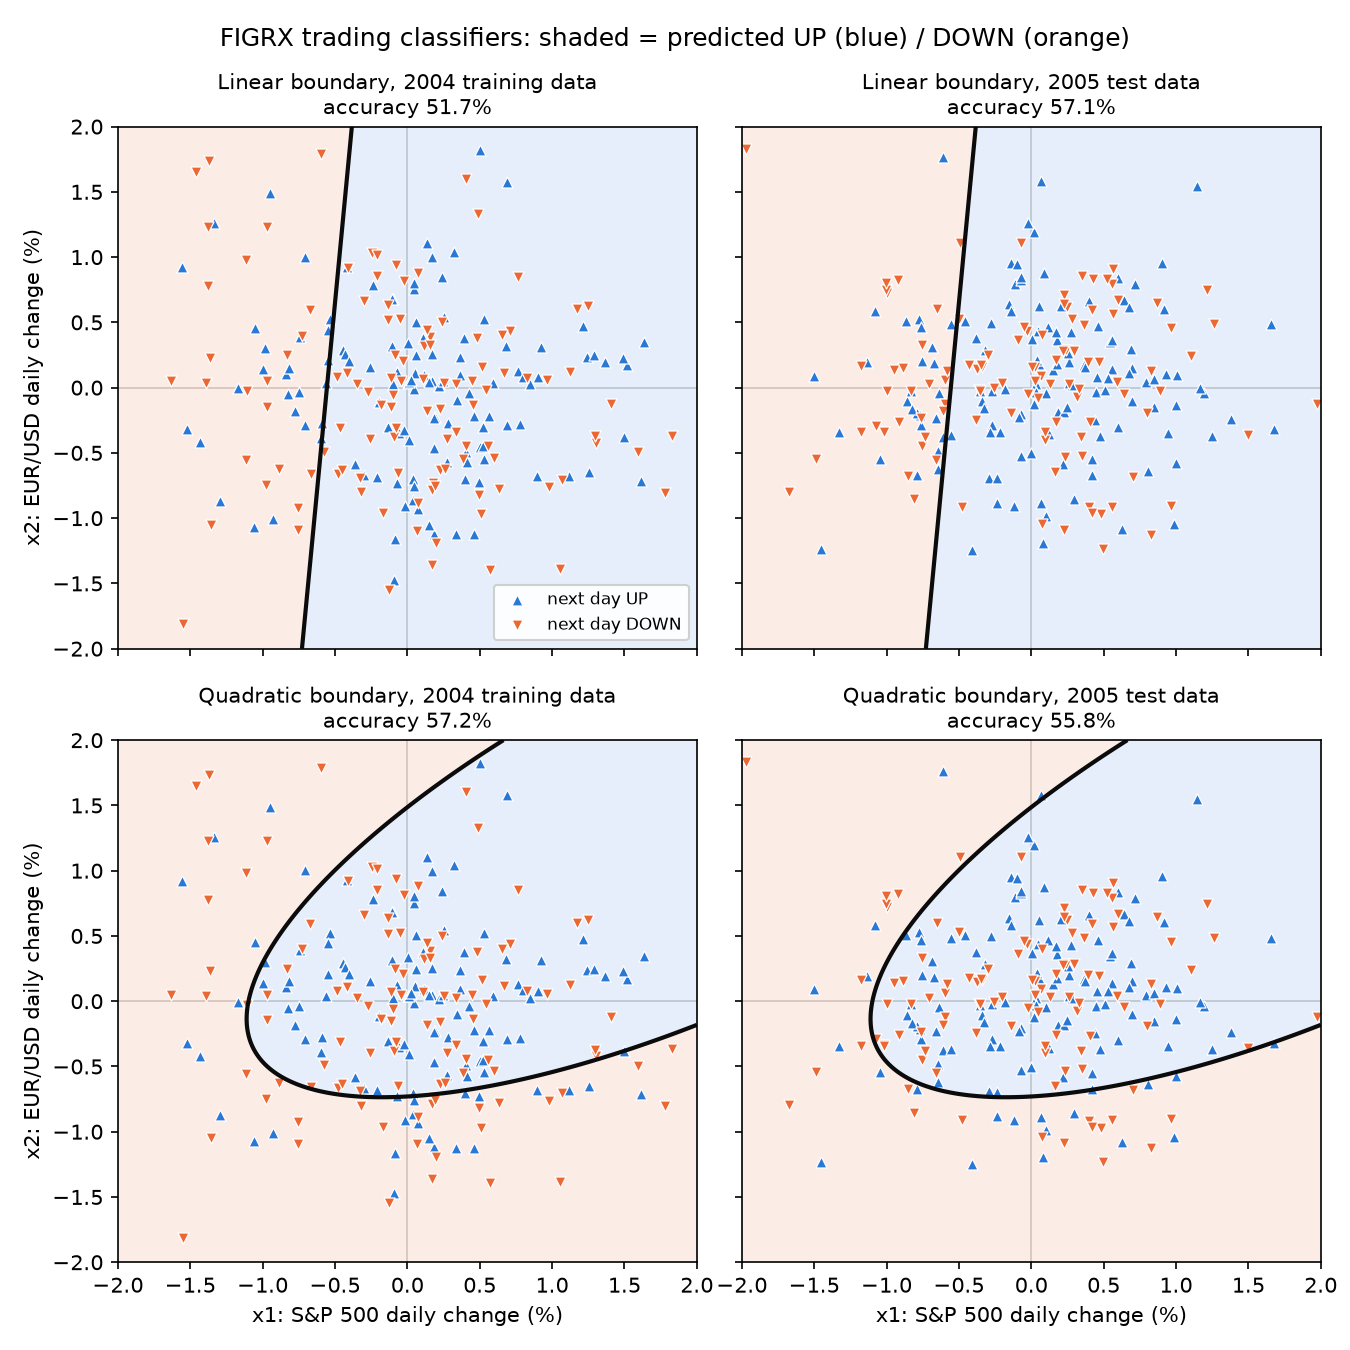
\includegraphics[width=0.8\linewidth]{p2_boundaries.png}
  \caption{Decision boundaries of the linear (top) and quadratic (bottom) classifiers over the 2004 training data
           (left) and the 2005 test data (right). Shading shows the predicted class; markers show the actual
           next-day FIGRX change.}
  \label{fig:p2boundaries}
\end{figure}

On 2005 days inside the ellipse, FIGRX rose the next day 56.6\% of the time, against 47.7\% outside. The outside
group holds 44 days, so its standard error is about 7.5 points, and the gap falls within sampling error. On the 2004
data used to fit the ellipse, the same comparison gave 56.7\% and 41.5\%.

\Needspace{14\baselineskip}
\subsection*{Trading results}
Each strategy holds FIGRX on days its classifier predicts UP and cash otherwise. Starting from \$1 million, I
compound the daily returns over the 2005 test period. GAIN is the cumulative return at the end of the year, and
EXPOSURE is the share of days invested in FIGRX.

\begin{center}\small
\begin{tabular}{lcc}
\toprule
Strategy & GAIN & EXPOSURE \\
\midrule
Linear & 21.81\% & 76.6\% \\
Quadratic & 15.19\% & 82.0\% \\
Buy-and-Hold & 14.92\% & 100.0\% \\
\bottomrule
\end{tabular}
\end{center}

Buy-and-Hold earns 14.92\%, from the January 4 close (27.55) to the December 30 close (31.66). The linear strategy
earns 6.9 points more while staying in cash on 57 days. On those days FIGRX moved $-0.10\%$ on average, against
$+0.11\%$ on the days the strategy held the fund. The gain depends on the size of each day's move, so a rule with a
small accuracy edge can earn more by skipping days with large declines. To judge luck, I drew 10{,}000 random strategies invested on the same 76.6\% of days. Their
median gain is 11.2\%, and 3.1\% of them reach 21.81\% or more.

\subsection*{Discussion}
\paragraph{(a) Can this strategy be used in practice?}
I would not trade my own money with it. The 2005 result rests on one test year, and I picked the better of two
models after seeing both. Neither classifier beats the always-UP rule in accuracy by more than the sampling error,
and the UP and DOWN days overlap across the input plane. A possible source of the linear rule's profit is the stale
pricing of international funds, whose prices use foreign closes that have not yet reacted to the US market; my
experiment does not test this mechanism. After the 2003 mutual-fund scandal, fund companies adopted fair-value
pricing, and many restrict short-term trading or charge redemption fees, which would close such a gap. The assignment
also assumes zero transaction costs. The linear strategy switches position 89 times in 2005. If each switch costs
0.1\% of the account, its gain falls from 21.81\% to 11.43\%, below the 14.92\% of Buy-and-Hold.

\paragraph{(b) VC-theoretical explanation.}
Problem 2 is a classification task with 0/1 loss, so the relevant result is the VC bound for classification. It
adds a confidence term $\Phi$ to the training error rate,
\[
  R(\omega) \le R_{\text{emp}}(\omega) + \Phi, \qquad
  \Phi = \sqrt{\frac{h\bigl(\ln(2n/h) + 1\bigr) - \ln(\eta/4)}{n}},
\]
and holds with probability at least $1 - \eta$. I set $\eta = \min(4/\sqrt{n}, 1)$, the textbook's practical rule,
which raises the confidence level as the sample grows. The multiplicative VC penalization factor used in Problem 1
belongs to regression. Each classifier is linear in its parameters, so its VC-dimension equals the parameter count:
$h = 3$ for the linear rule and $h = 6$ for the quadratic rule. A VC bound holds for every function in the model
set, so it also covers my least-squares classifiers, which do not minimize the 0/1 training error.

\begin{center}\small
\begin{tabular}{lcccccc}
\toprule
Classifier & $h$ & $n$ & $n/h$ & $R_{\text{emp}}$ & $\Phi$ & Upper bound on $R$ \\
\midrule
Linear & 3 & 236 & 78.7 & 0.483 & 0.298 & 0.781 \\
Quadratic & 6 & 236 & 39.3 & 0.428 & 0.385 & 0.813 \\
\bottomrule
\end{tabular}
\end{center}

The 0/1 training error uses the 236 days with a nonzero FIGRX change. With $n = 236$, the rule gives
$\eta = 4/\sqrt{236} \approx 0.26$, so the bounds hold with probability at least $1 - \eta \approx 74\%$, below the
95\% level common in statistics.

The textbook calls a sample small when $n/h$ is below about 15; in that regime $\Phi$ stays large, and model
selection has to match the complexity to the data. The
assignment fixes two low-capacity model sets in advance and fits each once, without searching over model sizes. Both
classifiers lie well above the small-sample threshold ($n/h$ of 78.7 and 39.3), which gives intuitive support for this
choice: further complexity control has less to gain here than in the small samples of Problem 1. This argument is a
heuristic, and a large $n/h$ leaves room for some benefit from complexity control.

Despite the large $n/h$, both upper bounds (0.781 and 0.813) exceed the 0.5 error of random guessing, so the theory
certifies no useful classifier from these 236 days. The training error rates sit near 0.5 before adding $\Phi$, and $\Phi$ needs a
large $n$ to become small, since its numerator also grows with $\ln n$. With $h = 3$ and the same rule for $\eta$,
$\Phi$ falls to about 0.06 only near $n = 10{,}000$ trading days.

The bound also assumes independent samples from one fixed distribution. Daily returns can depend on earlier days,
and the 2004 and 2005 markets need not share a distribution, so the bound gives a rough guide to the 2005 test error
at best. My results show that these two classifiers, with these two inputs, did not deliver a robust predictive
advantage in 2005; other models and other inputs remain untested.


\clearpage
% ============================================================
% Appendix of the combined HW2 report: reproducible numerical checks for Problem 1.
% Included from main.tex via % ============================================================
% Appendix of the combined HW2 report: reproducible numerical checks for Problem 1.
% Included from main.tex via % ============================================================
% Appendix of the combined HW2 report: reproducible numerical checks for Problem 1.
% Included from main.tex via \input{appendix}. Source: HW2/practice/p1_checks.py.
% ============================================================

\section*{Appendix: reproducing the numbers}
Four scripts in the folder \texttt{HW2/practice} print the numbers in this report. \texttt{p1\_mine.py} and
\texttt{p2\_mine.py} run the two experiments, print the result tables, and draw the figures. \texttt{p1\_checks.py}
prints the numerical checks below and the other Problem~1 values quoted in the text: the training-error example, the
penalty factors, and the DoF chosen in the worst realizations. \texttt{p2\_checks.py} prints the Problem~2 values the
main script leaves out: the alignment counts, the shape test for the ellipse, the next-day UP rates inside and
outside it, the mean FIGRX change on cash days, the gain after transaction costs, the sampling errors, and the
values of $\Phi$ for larger samples. The two check scripts save their output in \texttt{p1\_checks\_output.txt} and
\texttt{p2\_checks\_output.txt}.

\subsection*{Numerical checks for Problem 1}
I ran all scripts with Python 3.11.9, NumPy 2.4.6, and SciPy 1.17.1. All checks use the data generator and random seeds of the main experiment. A matrix counts as rank
deficient when NumPy's \texttt{matrix\_rank} returns fewer than DoF; its threshold is the largest singular value
times $\max(n, \text{DoF})$ times machine epsilon.
\begin{enumerate}
  \item \textbf{Rank.} 200 samples of $x \sim U[0,1]$ with $n = 30$ (seed 1); count of rank-deficient matrices for each
        candidate DoF.
  \item \textbf{Leverage formula.} One sine-squared sample with $n = 30$ (seed 0); leave-one-out MSE from the formula
        and from 30 explicit refits, for DoF 9, 13, 15, 17, and 19.
  \item \textbf{cv selections.} The 300 realizations of each setting (seed 0), with cv computed by my default rule and by
        explicit refits for every candidate DoF. I compare the selected DoF realization by realization, so ``the same''
        means an identical choice in every one of the 300 realizations.
  \item \textbf{Solvers.} The 15 realizations with the highest fpe risk for each data set at $n = 30$ (seed 0), refitted
        with the LAPACK drivers \texttt{gelsd} and \texttt{gelss} (SVD-based) and \texttt{gelsy} (QR with column
        pivoting) through SciPy's \texttt{lstsq} with its default cutoff; the output lists the risk under each driver.
\end{enumerate}
. Source: HW2/practice/p1_checks.py.
% ============================================================

\section*{Appendix: reproducing the numbers}
Four scripts in the folder \texttt{HW2/practice} print the numbers in this report. \texttt{p1\_mine.py} and
\texttt{p2\_mine.py} run the two experiments, print the result tables, and draw the figures. \texttt{p1\_checks.py}
prints the numerical checks below and the other Problem~1 values quoted in the text: the training-error example, the
penalty factors, and the DoF chosen in the worst realizations. \texttt{p2\_checks.py} prints the Problem~2 values the
main script leaves out: the alignment counts, the shape test for the ellipse, the next-day UP rates inside and
outside it, the mean FIGRX change on cash days, the gain after transaction costs, the sampling errors, and the
values of $\Phi$ for larger samples. The two check scripts save their output in \texttt{p1\_checks\_output.txt} and
\texttt{p2\_checks\_output.txt}.

\subsection*{Numerical checks for Problem 1}
I ran all scripts with Python 3.11.9, NumPy 2.4.6, and SciPy 1.17.1. All checks use the data generator and random seeds of the main experiment. A matrix counts as rank
deficient when NumPy's \texttt{matrix\_rank} returns fewer than DoF; its threshold is the largest singular value
times $\max(n, \text{DoF})$ times machine epsilon.
\begin{enumerate}
  \item \textbf{Rank.} 200 samples of $x \sim U[0,1]$ with $n = 30$ (seed 1); count of rank-deficient matrices for each
        candidate DoF.
  \item \textbf{Leverage formula.} One sine-squared sample with $n = 30$ (seed 0); leave-one-out MSE from the formula
        and from 30 explicit refits, for DoF 9, 13, 15, 17, and 19.
  \item \textbf{cv selections.} The 300 realizations of each setting (seed 0), with cv computed by my default rule and by
        explicit refits for every candidate DoF. I compare the selected DoF realization by realization, so ``the same''
        means an identical choice in every one of the 300 realizations.
  \item \textbf{Solvers.} The 15 realizations with the highest fpe risk for each data set at $n = 30$ (seed 0), refitted
        with the LAPACK drivers \texttt{gelsd} and \texttt{gelss} (SVD-based) and \texttt{gelsy} (QR with column
        pivoting) through SciPy's \texttt{lstsq} with its default cutoff; the output lists the risk under each driver.
\end{enumerate}
. Source: HW2/practice/p1_checks.py.
% ============================================================

\section*{Appendix: reproducing the numbers}
Four scripts in the folder \texttt{HW2/practice} print the numbers in this report. \texttt{p1\_mine.py} and
\texttt{p2\_mine.py} run the two experiments, print the result tables, and draw the figures. \texttt{p1\_checks.py}
prints the numerical checks below and the other Problem~1 values quoted in the text: the training-error example, the
penalty factors, and the DoF chosen in the worst realizations. \texttt{p2\_checks.py} prints the Problem~2 values the
main script leaves out: the alignment counts, the shape test for the ellipse, the next-day UP rates inside and
outside it, the mean FIGRX change on cash days, the gain after transaction costs, the sampling errors, and the
values of $\Phi$ for larger samples. The two check scripts save their output in \texttt{p1\_checks\_output.txt} and
\texttt{p2\_checks\_output.txt}.

\subsection*{Numerical checks for Problem 1}
I ran all scripts with Python 3.11.9, NumPy 2.4.6, and SciPy 1.17.1. All checks use the data generator and random seeds of the main experiment. A matrix counts as rank
deficient when NumPy's \texttt{matrix\_rank} returns fewer than DoF; its threshold is the largest singular value
times $\max(n, \text{DoF})$ times machine epsilon.
\begin{enumerate}
  \item \textbf{Rank.} 200 samples of $x \sim U[0,1]$ with $n = 30$ (seed 1); count of rank-deficient matrices for each
        candidate DoF.
  \item \textbf{Leverage formula.} One sine-squared sample with $n = 30$ (seed 0); leave-one-out MSE from the formula
        and from 30 explicit refits, for DoF 9, 13, 15, 17, and 19.
  \item \textbf{cv selections.} The 300 realizations of each setting (seed 0), with cv computed by my default rule and by
        explicit refits for every candidate DoF. I compare the selected DoF realization by realization, so ``the same''
        means an identical choice in every one of the 300 realizations.
  \item \textbf{Solvers.} The 15 realizations with the highest fpe risk for each data set at $n = 30$ (seed 0), refitted
        with the LAPACK drivers \texttt{gelsd} and \texttt{gelss} (SVD-based) and \texttt{gelsy} (QR with column
        pivoting) through SciPy's \texttt{lstsq} with its default cutoff; the output lists the risk under each driver.
\end{enumerate}


\end{document}
